% Chapter 4: Application Studies
\chapter{Application Studies}
\label{chapter:skelcl-evaluation}
\addtocontents{lof}{\protect\vspace{\beforebibskip}}%
\addtocontents{lol}{\protect\vspace{\beforebibskip}}%

\lettrine[lines=3, loversize=0.1]{I}{n this chapter} we present various application studies evaluating the usefulness and performance of the abstractions introduced by the \SkelCL programming model which were presented in the previous chapter.
We start with a brief discussion of the metrics used to evaluate the \SkelCL programming model and discuss the experimental setup used throughout the chapter.
We will then look at applications from a wide range of domains ranging from simple benchmark applications like the computation of the Mandelbrot set, over linear algebra and image processing applications, to real-world applications in medical imaging, and physics.

For all source codes we only show the relevant code sections and omit implementation details like initializing \SkelCL. %, including the correct set of header files, and prefix all symbols defined within the \code{skelcl} namespace.

\section{Experimental Setup}
\label{sec:skelcl:experimental_setup}
This section briefly discusses the evaluation metrics used in this chapter which were chosen to measure the quality of the abstractions introduced in the \SkelCL programming model and their implementation in the \SkelCL library.
We will also discuss the hardware used in the experiments.


\subsection{Evaluation Metrics}
We want to evaluate programmability, \ie, the ease of programming, and the performance of the \SkelCL programming model and library.

Measuring programmability is difficult.
Various studies~\cite{HochsteinCSAB2005,HochsteinBVG2008} have been conducted and metrics~\cite{VanderwielNL1997} have been proposed to measure how convenient a certain style of programming or a certain programming model is.
None of these metrics is widely established in the scientific or industrial communities.
We chose to use one of the simples metrics possible to quantify programming effort: counting the \emph{Lines Of source Code} (LOC).
The author wants to emphasize that this metric is not always a good representation of programmability.
A shorter program does not necessarily mean that the development of the program has been more convenient.
We will, therefore, alongside presenting the lines of code argue \emph{why} \SkelCL simplifies the programming of parallel devices, like \GPUs, as compared to the state-of-the-art approach \OpenCL.
% These discussions will argue that code written using the \SkelCL programming approach has, besides ease of programming, other properties of high quality software including:
% high level of re-use, portability, 

As the metric for performance we use absolute and relative runtime.
%-- where possible --
We only make comparisons using software executed on the same hardware.
We perform comparisons using published application and benchmark software from researchers or officially provided by Nvidia or AMD.
In addition, we compare self developed and optimized \OpenCL code versus code written using the \SkelCL library.

For all measurements we performed 100 runs and report the median runtime.

\subsection{Hardware Setup}
For performing our runtime experiments we used a PC equipped with a quad-core \CPU (Intel Xeon E5520, 2.26\,GHz) and 12\,GB of main memory.
The system is connected to a Nvidia Tesla S1070 computing system consisting of four Nvidia Tesla \GPUs.
The S1070 has 16\,GB of dedicated memory (4\,GB per \GPU) which is accessed with up to 408\,GB/s (102\,GB/s per \GPU).
Each \GPU comprises 240 streaming processor cores running at up to 1.44\,GHz.
The Linux based Ubuntu operating system was used.
The runtime experiments where conducted at different times from 2010 until 2015.
For each experiment the latest Nvidia \GPU driver available was used.

This hardware setup represents a common heterogeneous system comprising four \CPU cores and 960 \GPU streaming processor cores with a total of 28\,GB of memory.
Overall this system has a theoretical single-precision floating point performance of 4219.52 GFLOPS (4 $\times$ 1036.8 GFLOPS for the \GPUs and 72.32 GFLOPS for the \CPU).



\section{Mandelbrot}

\from{HIPS begin}
\subsection{HIPS}
The Mandelbrot~\cite{Mandelbrot-80} set are all complex numbers $c \in {\mathbb C}$ for which the sequence
\begin{equation}
	z_{i+1} = z_{i}^{2} + c, i\in {\mathbb N}
	\label{eq:mandelbrot}
\end{equation}
starting with $z_{0}=0$ does not escape to infinity.
If drawn as an image with each pixel representing a complex number, the boundary of the Mandelbrot set forms a fractal.
The calculation of such an image is a time-consuming task, because the sequence given by~(\ref{eq:mandelbrot}) has to be calculated for every pixel.
If this sequence does not cross a given threshold for a given number of steps, it is presumed that the sequence will converge.
The respective pixel is thus taken as a member of the Mandelbrot set, and it is painted black.
Other pixels outside are assigned a color that corresponds to the number of iterations of the sequence given by~(\ref{eq:mandelbrot}).
Computing a Mandelbrot fractal is easily parallelizable, as all pixels of the fractal can be computed simultaneously.

\subsubsection{Programming effort}
\label{sec:mandelbrot:implementation}

We created three similar parallel implementations for computing a Mandelbrot fractal using CUDA, OpenCL, and SkeCL.

CUDA and SkelCL require a single line of code for initialization in the host code, whereas OpenCL requires a lengthy creation and initialization of different data structures which take about 20 lines of code.

The host code differs significantly between all implementations.
In CUDA, the kernel is called like an ordinary function.
A proprietary syntax is used to specify the size of work-groups executing the kernel.
With OpenCL, several API functions are called to load and build the kernel, pass arguments to it and to launch it using a specified work-group size.
In SkelCL, the kernel passed to a newly created instance of a \texttt{Map} skeleton (see Section~\ref{sec:skeletons}).
A \texttt{Vector} of complex numbers, each of which is represented by a pixel of the Mandelbrot fractal, is passed to the \texttt{Map} skeleton upon execution.
Specifying the work-group size is mandatory in CUDA and OpenCL, whereas this is optional in SkelCL.
However, it is sometimes reasonable to also hand-optimize the work-group size in SkelCL, since it can have a considerable impact on performance.

\paragraph{Program size}
The OpenCL-based implementation has 118 lines of code (kernel: 28~lines, host program: 90~lines) and is thus more than twice as long as the CUDA and SkelCL versions with 49 lines (28, 21) and 57 lines (26, 31), respectively (see Figure~\ref{fig:mandelbrot_runtime}).
The length of the CUDA- and SkelCL-based implementations differs by only a few lines.

\paragraph{Kernel size}
The kernel function is similar in all implementations: it takes a pixel's position (i.e., a complex number) as input, performs the iterative calculation for this pixel, and returns the pixel's color.
However, while the input positions have to be given explicitly when using the \texttt{Map} skeleton in SkelCL, no positions are passed to the kernel in the CUDA- and OpenCL-based implementations.

\subsubsection{Performance experiments}
\label{sec:mandelbrot:runtime}

\begin{figure}[bp]
    \centering
    \includegraphics[width=0.42\textwidth]{HIPS/ChartMandelbrot}
    \caption{Runtime and program size of the Mandelbrot application.}
    \label{fig:mandelbrot_runtime}
\end{figure}%


We tested our implementations on a single GPU of our test system to compute a Mandelbrot fractal of size 4096$\times$3072 pixels.
In CUDA and OpenCL, work-groups of 16$\times$16 are used; SkelCL uses its default work-group size of~256.
The results are shown in Figure~\ref{fig:mandelbrot_runtime}.
As compared to the runtime of the SkelCL-based implementation (26 seconds), the implementation based on OpenCL (25 seconds) and CUDA (18 seconds) are faster by 4\% or 31\%, respectively.
Since SkelCL is built on top of OpenCL, the performance difference of SkelCL and OpenCL can be regarded as the overhead introduced by SkelCL\@.
Previous work~\cite{KoDYLCSMZ-10} also reported that CUDA was usually faster than OpenCL, which also explains the higher performance of the implementation based on CUDA.
The Mandelbrot application demonstrates that SkelCL introduces a tolerable overhead of less than 5\% as compared to OpenCL.
A clear benefit of this overhead is the reduced programming effort required by the SkelCL programm.
\from{HIPS end}


\from{PaCT begin}
\subsection{Application Study: Mandelbrot Set (PaCT)}
\label{sec:mandelbrot}

The Mandelbrot set calculation~\cite{Mandelbrot-80} is a time-consuming task which is often used as a benchmark. Computing a Mandelbrot fractal is easily parallelizable, as all pixels can be computed simultaneously.
As the criteria for programming effort we use the number of Lines of Code (LoC), the results are in Fig.~\ref{fig:mandelbrot_runtime}. 

We created three similar parallel implementations for computing a Mandelbrot fractal using CUDA, OpenCL, and SkeCL.

CUDA and SkelCL require a single line of code for initialization in the host code, whereas OpenCL requires a
\begin{figure}
    \centering
    \includegraphics[width=0.6\textwidth]{PaCT/mandelbrotChartFinal.pdf}
    \caption{Runtime and program size of the Mandelbrot application.}
    \label{fig:mandelbrot_runtime}
\end{figure}%
lengthy creation and initialization of different data structures which take about 20 LoC.
The host CPU code differs significantly between all implementations.
In CUDA, the kernel is called like an ordinary function.
A proprietary syntax is used to specify the size of work-groups executing the kernel.
In OpenCL, several API functions are called to load and build the kernel, pass arguments to it and launch it using a specified work-group size.
In SkelCL, the kernel is passed to a newly created instance of the \texttt{Map} skeleton.
A \texttt{Vector} of complex numbers, each of which represents a pixel of the Mandelbrot fractal, is passed to the \texttt{Map} skeleton upon execution.
Specifying the work-group size is mandatory in CUDA and OpenCL, whereas this is optional in SkelCL.

The OpenCL-based implementation has in total 118 lines of code (kernel: 28~lines, host program: 90~lines) and is thus more than twice as long as the CUDA and SkelCL versions with 49 lines (28, 21) and 57 lines (26, 31), respectively (see Figure~\ref{fig:mandelbrot_runtime}).

We tested our implementations on a single GPU of our test system to compute a Mandelbrot fractal of size 4096$\times$3072 pixels.
In CUDA and OpenCL, work-groups of 16$\times$16 are used; SkelCL uses its default work-group size of~256.

As compared to the runtime of the SkelCL-based implementation (26 sec), the implementation based on OpenCL (25 sec) and CUDA (18 sec) are faster by 4\% or 31\%, respectively.
Since SkelCL is built on top of OpenCL, the performance difference of SkelCL and OpenCL can be regarded as the overhead introduced by SkelCL\@.
Previous work~\cite{KoDYLCSMZ-10} reported that CUDA was usually faster than OpenCL, which explains the higher performance of the implementation based on CUDA.
The Mandelbrot application demonstrates that SkelCL introduces a tolerable overhead of less than 5\% as compared to OpenCL.

\from{PaCT end}


\section{Linear Algebra Applications}

  \subsection{Sum of absolute values}

  \subsection{Dot product}

  \section{Matrix Multiplication}
\label{section:skelcl:matrixMult}

The multiplication of matrices is a fundamental building block for many scientific applications.
A $n\times d$ matrix $A$ is multiplied with a $d\times m$ matrix $B$ to produce a $n\times m$ matrix $C$, where the elements of $C$ are computed as:
\begin{equation*}
  C_{ij} = \sum_{k=0}^{d} A_{ik} \times B_{kj}, \qquad \forall\ i \in 1, \ldots, n \wedge j \in 1, \ldots, m
\end{equation*}
Here $A_{i*}$ refers to the $i$th row of $A$ and $B_{*j}$ to the $j$th column of $B$.
\autoref{fig:mm} visualizes this computation.
To compute the highlighted element in matrix $C$, the highlighted row of matrix $A$ is combined with the highlighted column of matrix $B$.
For computing the entire matrix $C$, \emph{all pairs} of rows from $A$ and columns of $B$ have to be processed.
Therefore, in \SkelCL the \allpairs skeleton can be used to express matrix multiplication.

\begin{figure}[tb]
  \centering
  \includegraphics[width=0.5\textwidth]{HLPP/mm}
  \caption[Visalization of matrix multiplication.]%
          {Matrix multiplication $A\times B = C$.
           The red highlighted element in matrix $C$ is computed by combining the highlighted row of matrix $A$ with the highlighted column of matrix $B$.}
  \label{fig:mm}
\end{figure}


\subsubsection*{\SkelCL Implementation}
\autoref{eq:skelcl:mm} shows how matrix multiplication can be expressed using the \allpairs skeleton in the \SkelCL programming model:
\begin{align}
  \label{eq:skelcl:mm}
  mm\ A\ B &= allpairs\ f\ A\ B^T\\
  \text{where:} \qquad f\ \vec{a}\ \vec{b} &= \sum_{k=0}^d a_k \times b_k \nonumber
\end{align}
When looking back at \autoref{eq:dot_product} in the previous section, we can see, that $f$ is actually the dot product computation, therefore, we can write:
\begin{align}
  mm\ A\ B &= allpairs\ dotProduct\ A\ B^T
  \label{eq:skelcl:mm:dot}
\end{align}
We know that we can express the dot product as a sequential composition of the \zip and \reduce skeletons as we saw in the previous section.
In \autoref{chapter:skelcl}, \autoref{section:skelcl-programming-model:specialSkeletons}, we discussed a specialized implementation of the \allpairs skeleton for computations which can be expressed in this way.
Therefore, we can use the \SkelCL library to develop two implementations:
1) using the generic \allpairs skeleton; and 2) using the specialized \allpairs skeleton.

\autoref{lst:skelcl:mm:generic} shows the implementation of matrix multiplication using the generic \allpairs skeleton.
\begin{lstlisting}[%                                                             
caption={Implementation of matrix multiplication using the generic \allpairs skeleton in \SkelCL.},%
numbers=left,%
float=tb,
label={lst:skelcl:mm:generic}]
Matrix<float> mm(const Matrix<float>& A,$\label{lst:skelcl:mm:generic:CPU:start}$
                 const Matrix<float>& B) {
  skelcl::init();
  auto mm = allpairs($\label{lst:skelcl:mm:generic:CPU:stop}$
    [](const Vector<float>& a, const Vector<float>& b) {$\label{lst:skelcl:mm:generic:GPU:start}$
      float c = 0.0f;
      for (int i = 0; i < a.size(); ++i)
        c += a[i] * b[i];
      return c; });$\label{lst:skelcl:mm:generic:GPU:stop}$
  return mm(A, B); }$\label{lst:skelcl:mm:generic:CPU:call}$
\end{lstlisting}
The skeleton is customized with a lambda expression processing two vectors:
$a$ is a row vector of matrix $A$ and $b$ is a column vector of matrix $B$.
In this generic implementation the dot product computation is implemented using a \code{for} loop iterating over the vectors, multiplying elements pairwise and summing them up in the accumulation variable $c$.

\autoref{lst:skelcl:mm:special} shows the implementation of matrix multiplication using the specialized \allpairs skeleton.
\begin{lstlisting}[%                                                             
caption={Implementation of matrix multiplication using the specialized \allpairs skeleton in \SkelCL.},%
float=tb,%                                                                       
numbers=left,%
label={lst:skelcl:mm:special}]
Matrix<float> mm(const Matrix<float>& A,
                 const Matrix<float>& B) {
  skelcl::init();
  auto mult  = zipVector($\label{lst:skelcl:mm:special:zip}$
      [](float x, float y){return x*y;});$\label{lst:skelcl:mm:special:zipGPU}$
  auto sumUp = reduce($\label{lst:skelcl:mm:special:reduce}$
      [](float x, float y){return x+y;}, 0);$\label{lst:skelcl:mm:special:reduceGPU}$
  auto mm    = allpairs(sumUp, mult);
  return mm(A, B); }
\end{lstlisting}
Here the \allpairs skeleton is customized with \zip and \reduce skeletons defined in \autoref{lst:skelcl:mm:special:zip} and \autoref{lst:skelcl:mm:special:reduce}.
This implementation corresponds more closely to \autoref{eq:skelcl:mm:dot}:
as we express the dot product using these two skeletons (as shown in \autoref{eq:skelcl:dot_product}).
Therefore, we reuse the definitions of \code{mult} and \code{sumUp} as used in \autoref{lst:skelcl:dot}.

\subsubsection*{Implementations used for comparison}
We compare six different implementations of matrix multiplication:
\begin{enumerate}
  \item the \OpenCL implementation from~\cite{KirkHw2010} without optimizations,
  \item the optimized \OpenCL implementation from~\cite{KirkHw2010} using \GPU local memory,
  \item the optimized \BLAS implementation by AMD~\cite{APPML} written in \OpenCL (\clBLAS version 1.10),
  \item the optimized \BLAS implementation by Nvidia~\cite{cuBLAS} written in \CUDA (\CUBLAS version 5.0),
  \item the \SkelCL implementation using the generic \allpairs skeleton shown in \autoref{lst:skelcl:mm:generic},
  \item the \SkelCL implementation using the specialized \allpairs skeleton shown in \autoref{lst:skelcl:mm:special}.
\end{enumerate}

\paragraph{1. OpenCL implementation}
\autoref{lst:naive_opencl} shows the kernel of the first, unoptimized \OpenCL implementation from~\cite{KirkHw2010}.
\begin{lstlisting}[%                                                             
postbreak=\space, breakautoindent=true, breakindent=78pt, breaklines,
caption={[\OpenCL kernel of matrix multiplication without optimizations.]\OpenCL kernel of matrix multiplication without optimizations~\cite{KirkHw2010}.},%
float=tb,%
numbers=left,%
label={lst:naive_opencl}]
kernel void mm(global float* A, global float* B,        global float* C, int m, int d, int n) {
  int row = get_global_id(0);
  int col = get_global_id(1);
  float sum = 0.0f;
  for (int k = 0; k < d; k++)
    sum += A[row * d + k] * B[k * n + col];
  C[row * n + col] = sum; }
\end{lstlisting}

\vspace{-.5em}
\paragraph{2. Optimized OpenCL implementations}
The kernel of the optimized \OpenCL implementation from~\cite{KirkHw2010} using local memory is shown in \autoref{lst:local_mem_opencl}.
\begin{lstlisting}[%                                                             
postbreak=\space, breakautoindent=true, breakindent=78pt, breaklines,
caption={[\OpenCL kernel of the optimized matrix multiplication usgin local memory.]\OpenCL kernel of the optimized matrix multiplication using local memory~\cite{KirkHw2010}.},%
float=tb,%
numbers=left,%
label={lst:local_mem_opencl}]
#define T_WIDTH 16
kernel void mm(global float* A, global float* B,        global float* C, int m, int d, int n) {
  local float Al[T_WIDTH][T_WIDTH];$\label{lst:local_mem_opencl:allocA}$
  local float Bl[T_WIDTH][T_WIDTH];$\label{lst:local_mem_opencl:allocB}$
  int row = get_global_id(0);
  int col = get_global_id(1);
  int l_row = get_local_id(0);
  int l_col = get_local_id(1);
  float sum = 0.0f;
  for (int m = 0; m < d / T_WIDTH; ++m {$\label{lst:local_mem_opencl:loop}$
    Al[l_row][l_col] = A[row * d + (m * T_WIDTH + l_col)];$\label{lst:local_mem_opencl:loadA}$
    Bl[l_row][l_col] = B[(m * T_WIDTH + l_row) * d + col];$\label{lst:local_mem_opencl:loadB}$
    barrier(CLK_LOCAL_MEM_FENCE);$\label{lst:local_mem_opencl:barrier1}$
    for (int k = 0; k < T_WIDTH; k++)
      sum += Al[l_row][k] * Bl[k][l_col];$\label{lst:local_mem_opencl:comp}$
    barrier(CLK_LOCAL_MEM_FENCE); }$\label{lst:local_mem_opencl:barrier2}$
  C[row * n + col] = sum; }
\end{lstlisting}
Two fixed-sized arrays of local memory are allocated in \autoref{lst:local_mem_opencl:allocA} and \autoref{lst:local_mem_opencl:allocB}.
Matrix multiplication is carried out in the loop starting in \autoref{lst:local_mem_opencl:loop}.
In each iteration, data is loaded into the local memory (\autoref{lst:local_mem_opencl:loadA} and \autoref{lst:local_mem_opencl:loadB}) before it is used in the computation in \autoref{lst:local_mem_opencl:comp}.
Note that two synchronization barriers are required (\autoref{lst:local_mem_opencl:barrier1} and \autoref{lst:local_mem_opencl:barrier2}) to ensure that the data is fully loaded into the local memory and that the data is not overwritten while other work-items are still using it.

Both \OpenCL implementations 1. and 2. from~\cite{KirkHw2010} are restrictive:
they are only capable of performing matrix multiplication for square matrices.

\vspace{-.5em}
\paragraph{3. BLAS implementation by AMD}
The implementation offered by AMD is called \clBLAS, written in \OpenCL and is part of their Accelerated Parallel Processing Math Libraries (APPML)~\cite{APPML}.

\vspace{-.5em}
\paragraph{4. BLAS implementation by Nvidia}
\CUBLAS~\cite{cuBLAS} is implemented using \CUDA and, therefore, can only be used on \GPUs built by Nvidia.

\subsubsection*{Programming effort}
\autoref{fig:mat_mult_loc} shows the comparison regarding the number of lines of code (LOCs) required for each of the six implementations.
\autoref{tab:mat_mult_loc} presents the detailed numbers.
We did not count those LOCs which are not relevant for parallelization and are similar in all six implementations, like initializing the input matrices with data and checking the result for correctness.
For every implementation, we distinguish between \CPU (host) code and \GPU (kernel) code.


\begin{figure}[p]
  \begin{minipage}{\textwidth}
  \centering
  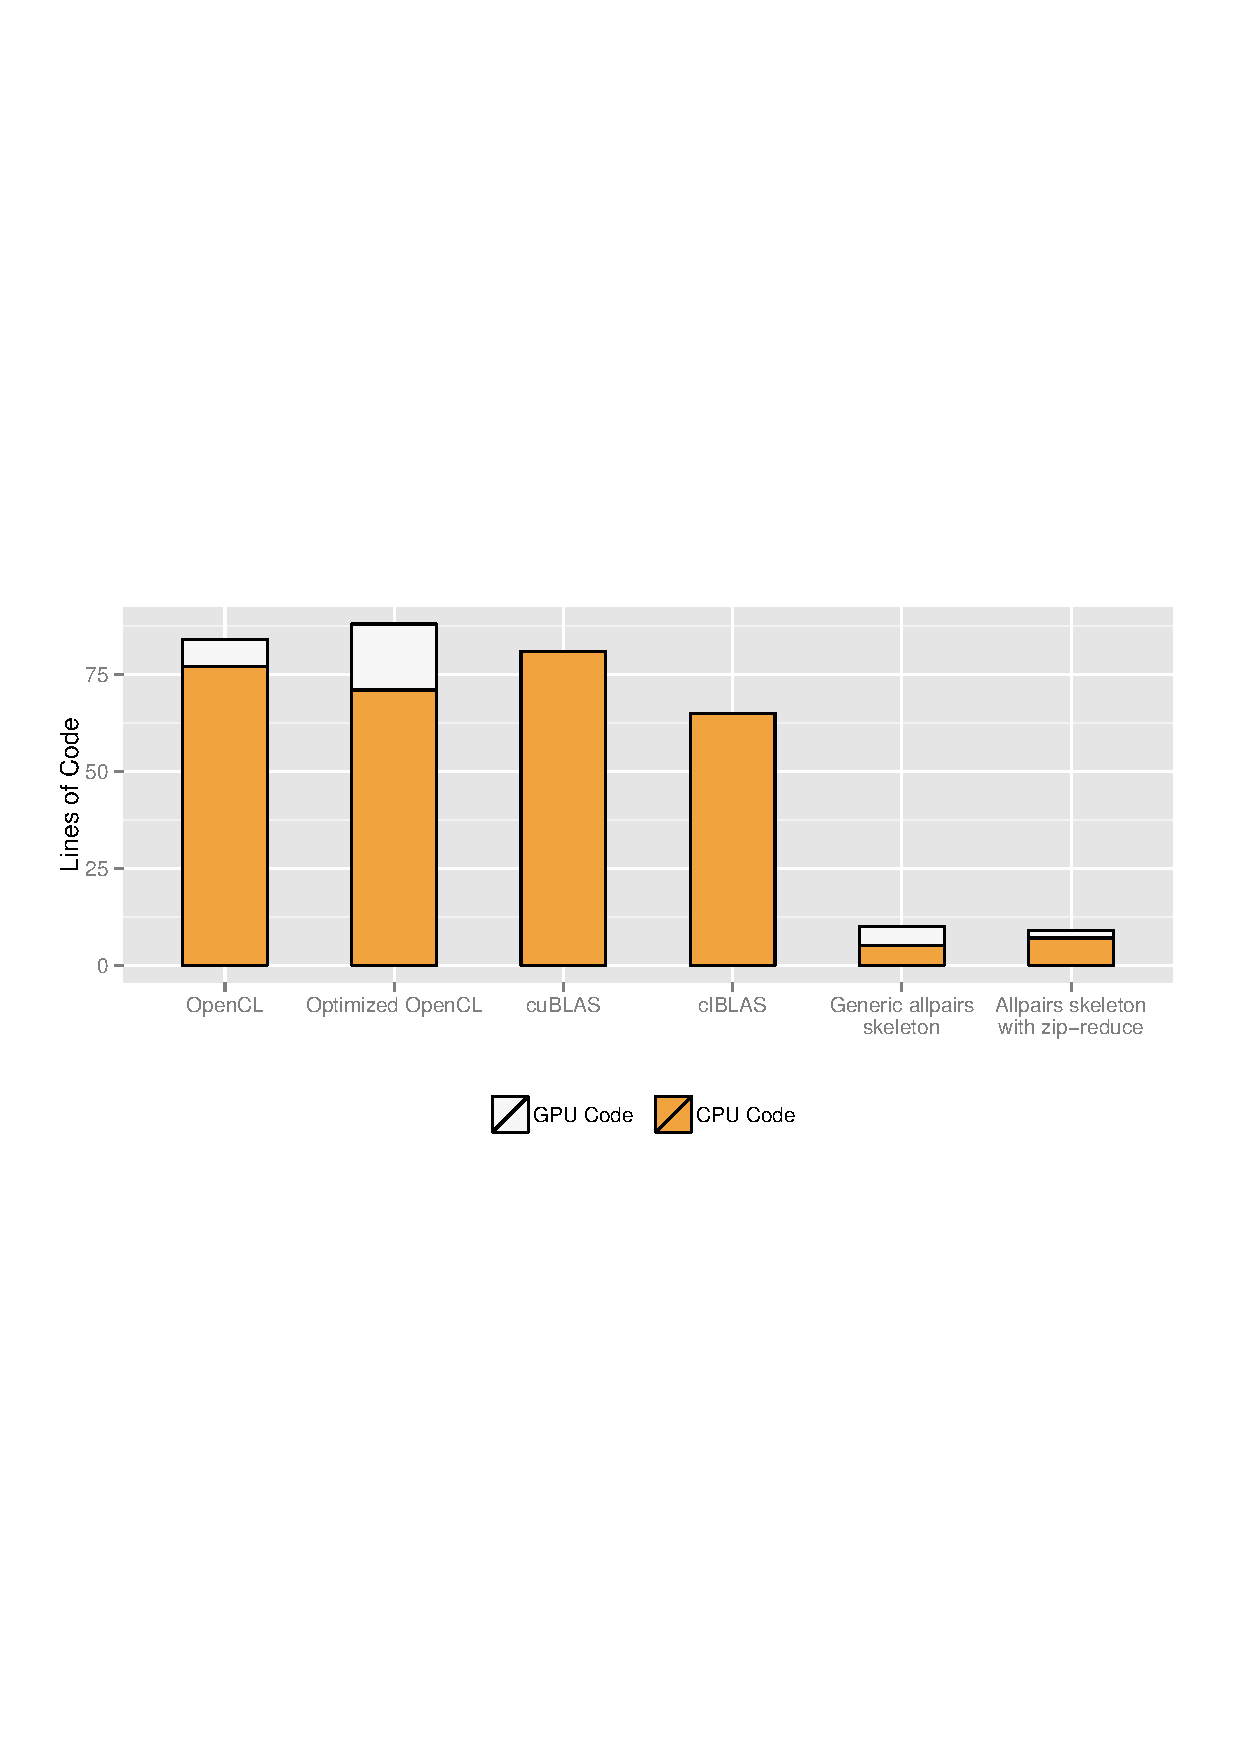
\includegraphics[width=\textwidth]{Plots/MatMult/mat_mult_loc}
  \caption[Programming effort of three \OpenCL-based, one \CUDA-base, and two \SkelCL-based matrix multiplication implementations.]%
          {Programming effort (Lines of Code) of three \OpenCL-based, and one \CUDA-based vs. two \SkelCL-based implementations.}
  \label{fig:mat_mult_loc}
  \end{minipage}
%\end{figure}
%\begin{table}[tb]
\strut\\[2em]\strut
  \begin{minipage}{\textwidth}
  \centering
  \begin{tabular}{lrrr}
    \toprule
              & \multicolumn{3}{c}{Lines of Code} \\
    \cmidrule(r){2-4}
    Implementation & \CPU & \GPU & Total \\[.5em]
    \midrule
    \OpenCL           & 77 &  7 & 84 \\[.5em]
    Optimized \OpenCL & 77 & 17 & 94 \\[.5em]
    \CUBLAS           & 81 & -- & 81\\[.5em]
    \clBLAS           & 65 & -- & 65\\[.5em]
    Generic \allpairs skeleton & 5 & 5 & 10\\[.5em]
    Specialized \allpairs skeleton & 7 & 2 & 9\\[.5em]
    \bottomrule
  \end{tabular}
  \captionof{table}%
          [Lines of Code for matrix multiplication implementaitons.]%
          {Lines of Code of all compared implementations.}
  \label{tab:mat_mult_loc}
  \end{minipage}
%\end{table}
\end{figure}

In the \OpenCL implementations, the \GPU code includes the kernel definition, as shown in \autoref{lst:naive_opencl} and \autoref{lst:local_mem_opencl};
the \CPU code includes the initialization of \OpenCL, memory allocations, explicit data transfer operations, and management of the execution of the kernel.

In the \BLAS implementations, the \CPU code contains the initialization of the corresponding \BLAS library, memory allocations, as well as a library call for performing the matrix multiplication;
no separate definition of \GPU code is necessary, as the \GPU code is defined inside the library function calls.

For the implementation based on the generic \allpairs skeleton (\autoref{lst:skelcl:mm:generic}), we count \autoref{lst:skelcl:mm:generic:CPU:start}---\autoref{lst:skelcl:mm:generic:CPU:stop} and \autoref{lst:skelcl:mm:generic:CPU:call} as the \CPU code, and the definition of the customizing function in \autoref{lst:skelcl:mm:generic:GPU:start}---\autoref{lst:skelcl:mm:generic:GPU:stop} as the \GPU code.
For the implementation based on the specialized \allpairs skeleton (\autoref{lst:skelcl:mm:special}), \autoref{lst:skelcl:mm:special:zipGPU} and \autoref{lst:skelcl:mm:special:reduceGPU} are the \GPU code, while all other lines constitute the \CPU code.

Both skeleton-based implementations are clearly the shortest, with 10 and 9 LOCs.
The next shortest implementation is the \CUBLAS implementation with 65 LOCs -- 7 times longer than the \SkelCL-based implementations.
The other implementations using \OpenCL require even 9 times more LOCs than the \SkelCL-based implementations.

Besides their length, the \OpenCL-based implementations require the application developer to explicitly implement many low-level, error-prone tasks, like dealing with pointers and offset calculations.
Furthermore, the skeleton-based implementations are more general, as they can be used for arbitrary allpairs computations, while all other implementations can compute matrix multiplication only.


\subsubsection*{Performance experiments}
We performed experiments with the six different implementations of matrix multiplication on two different computer systems with \GPUs:
\begin{itemize}[leftmargin=50pt]
  \item[System A:] Our general testing system already described in~\autoref{sec:skelcl:experimental_setup}:
    an Nvidia S1070 equipped with four Nvidia Tesla \GPUs, each with 240 streaming processors and 4 GByte memory.
  \item[System B:] An AMD Radeon HD 6990 card containing two \GPUs, each with 1536 streaming processors and 1 GByte memory.
\end{itemize}

\noindent
We include the data transfer times to and from the \GPU in the results. %, \ie the measured runtime consists of:
% 1) uploading the two input matrices to the \GPU;
% 2) performing the actual matrix multiplication;
% 3) downloading the computed result matrix.


\begin{figure}[tb]
  \centering
  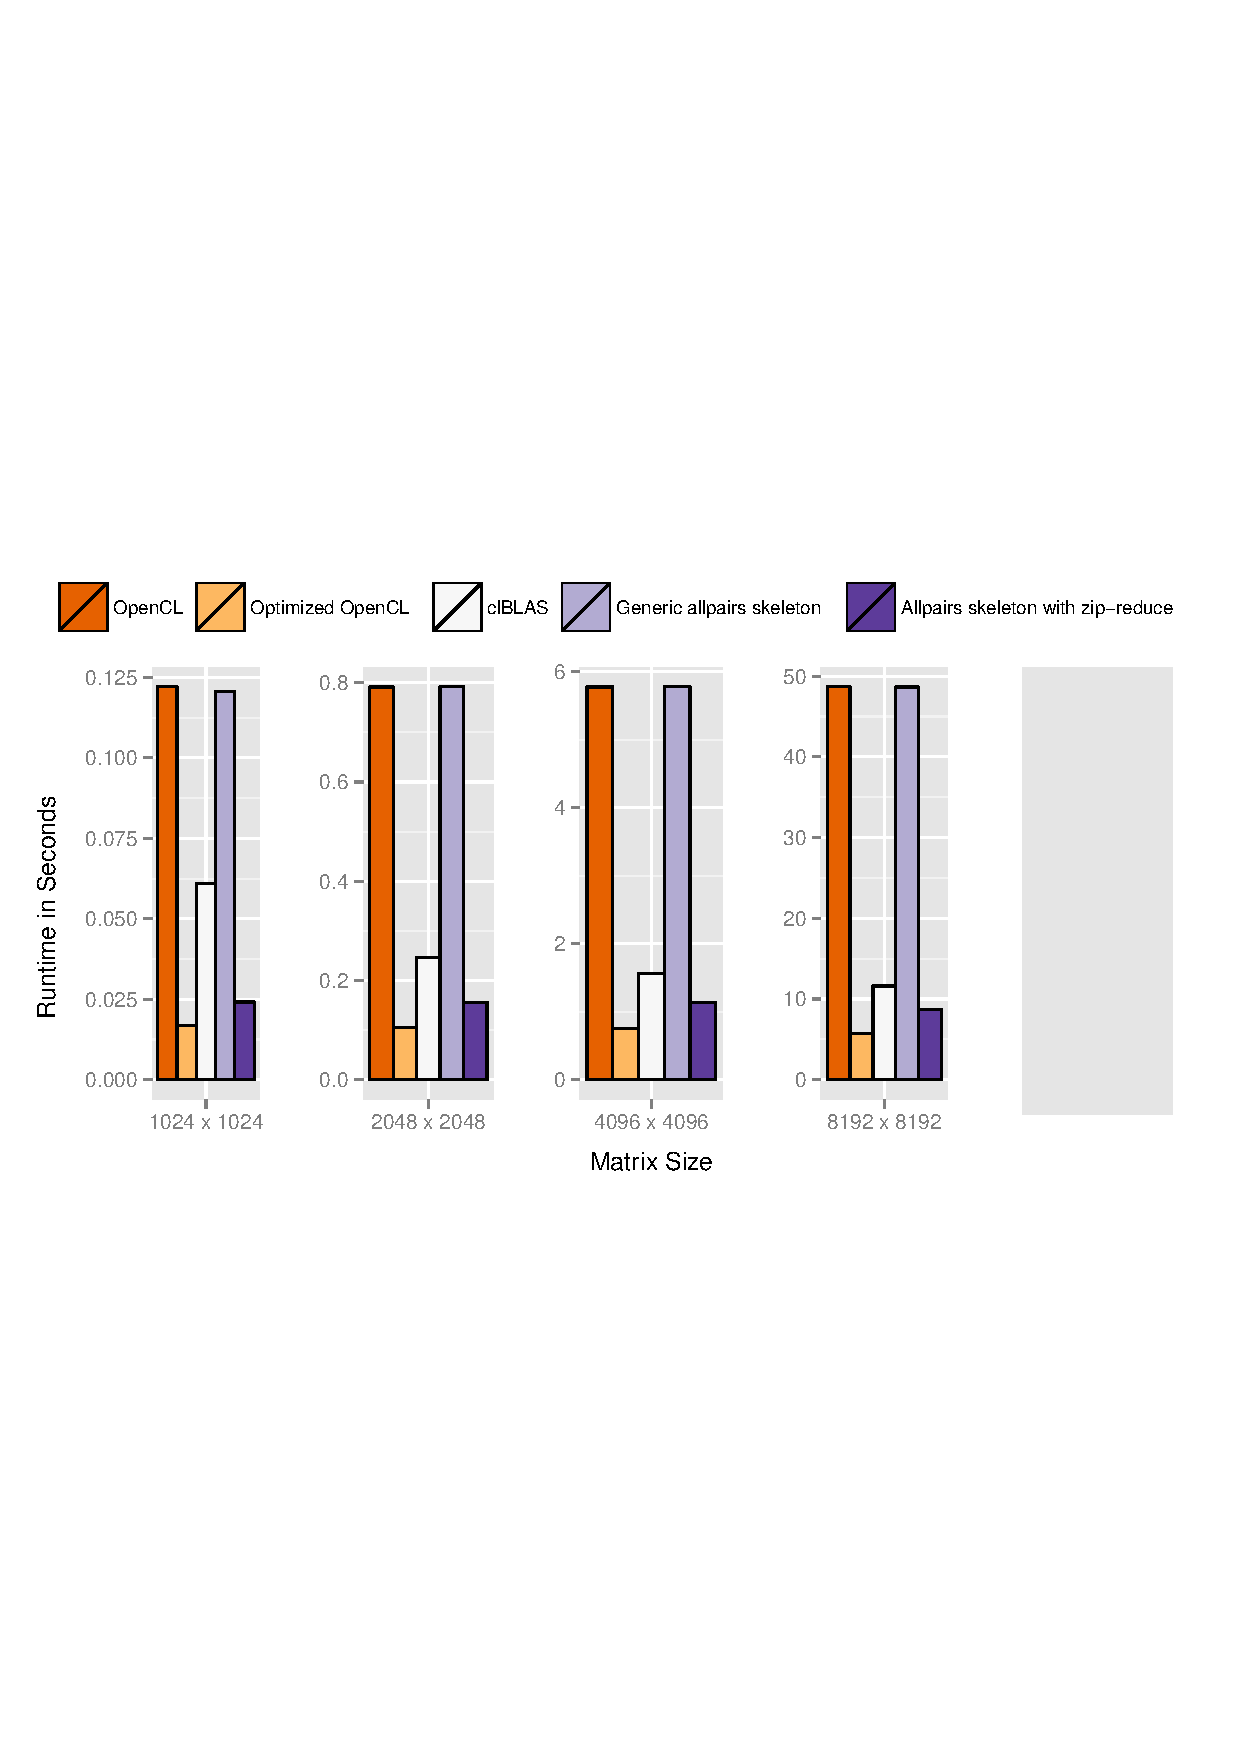
\includegraphics[width=0.8\textwidth]{Plots/MatMult/mat_mult_sizes_gtx480}
  \caption[Runtime of different matrix multiplication implementations on an Nvidia system.]%
          {Runtime of different matrix multiplication implementations on the Nvidia system for different sizes of the matrices.}
  \label{fig:mat_mult_single}
\end{figure}
\begin{table}[tb]
  \centering
  \begin{tabular}{lrrrrr}
    \toprule
              & \multicolumn{5}{c}{Runtimes in Seconds} \\
    \cmidrule(r){2-6}
    \multirow{2}{*}{Implementation} & $1024$ & $2048$ & $4096$ & $8192$ & $16384$ \\
                                    & $\times 1024$ & $\times 2048$ & $\times 4096$ & $\times 8192$ & $\times 16384$\\
    \midrule
    \OpenCL            & 0.122 & 0.791 & 5.778 & 48.682 & 472.557 \\
    Optimized \OpenCL  & 0.017 & 0.105 & 0.752 &  5.683 &  51.337 \\
    \CUBLAS            & 0.012 & 0.059 & 0.387 &  2.863 &  22.067 \\
    \clBLAS            & 0.061 & 0.246 & 1.564 & 11.615 &  90.705 \\
    Generic \allpairs  & \multirow{2}{*}{0.121} & \multirow{2}{*}{0.792} & \multirow{2}{*}{5.782} & \multirow{2}{*}{48.645} & \multirow{2}{*}{471.235} \\[-.5em]
    skeleton\\
    Specialized \allpairs & \multirow{2}{*}{0.024} & \multirow{2}{*}{0.156} & \multirow{2}{*}{1.134} & \multirow{2}{*}{8.742} & \multirow{2}{*}{68.544} \\[-.5em]
    skeleton\\
    \bottomrule
  \end{tabular}
  \caption[Runtime results for matrix multiplication on an Nvidia system.]
          {Runtime results for matrix multiplication on the Nvidia system.}
  \label{tab:mat_mult_single}
\end{table}

\paragraph{System A (one \GPU)}
\autoref{fig:mat_mult_single} shows the runtime of all six implementations for different sizes of the matrices (for readability reasons, all charts are scaled differently).
For detailed numbers, see \autoref{tab:mat_mult_single}.

Clearly, the naive \OpenCL implementation and the implementation using the generic \allpairs skeleton are the slowest, because both do not use local memory, in contrast to all other implementations.

The implementation using the specialized \allpairs skeleton performs 5.0 to 6.8 times faster than the generic allpairs skeleton, but is 33\% slower on the largest matrices than the optimized \OpenCL-based implementation. % using local memory.
However, the latter implementation can only be used for square matrices and, therefore, it benefits from omitting many conditional statements and boundary checks.


\CUBLAS is the fastest of all implementations, as it is highly tuned specifically for Nvidia \GPUs using \CUDA.
The \clBLAS implementation by AMD using \OpenCL performs not as well:
presumably, it is optimized for AMD \GPUs and performs poorly on other hardware.
Our optimized \allpairs skeleton implementation outperforms the \clBLAS implementation for all matrix sizes tested.


\pagebreak

\paragraph{System B (one \GPU)}
\autoref{fig:mat_mult_single_amd} shows the measured runtime in seconds for five of the six implementations for different sizes of the matrices.
Detailed numbers can be found in \autoref{tab:mat_mult_single_amd}.
We could not use the Nvidia-specific \CUBLAS implementation as it does not work on the AMD \GPU.

For bigger matrices, the slowest implementations are, again, the unoptimized \OpenCL implementation and the implementation using the generic \allpairs skeleton.

The optimized \OpenCL implementation and the specialized \allpairs skeleton perform similarly.
For matrices of size $8192\times 8192$, the optimized \OpenCL implementation is about 30\% faster.

The \clBLAS implementation performs very poorly for small matrices, but is clearly the fastest implementation for bigger matrices.
Similar to the \CUBLAS implementation on the Nvidia hardware, it is not surprising that the implementation by AMD performs very well on their own hardware.

\begin{figure}[tb]
  \centering
  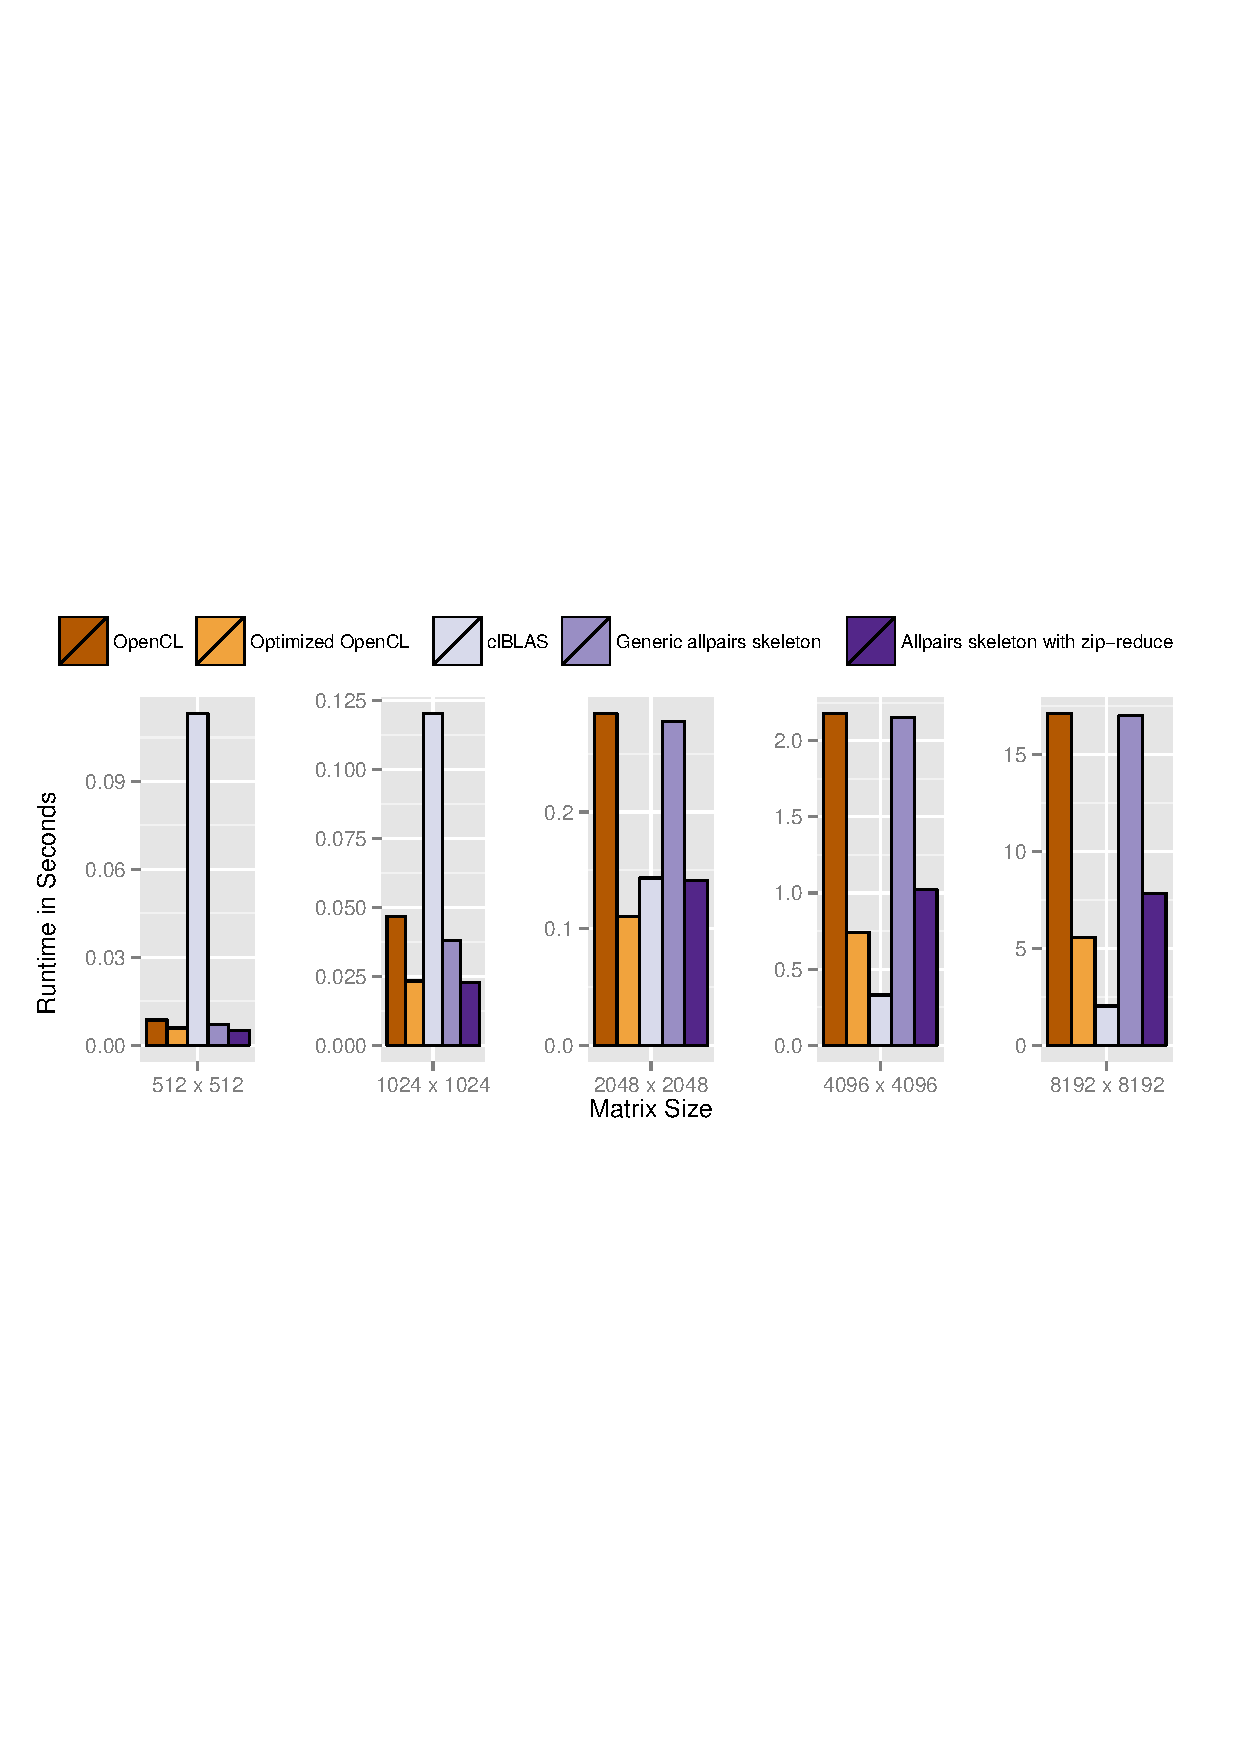
\includegraphics[width=0.8\textwidth]{Plots/MatMult/mat_mult_sizes_hd6990}
  \caption[Runtime of different matrix multiplication implementations on an AMD ststem.]%
          {Runtime of all compared implementations for a matrix multiplication on the AMD system using one \GPU.}
  \label{fig:mat_mult_single_amd}
\end{figure}
\begin{table}[tb]
  \centering
  \begin{tabular}{lrrrrr}
    \toprule
              & \multicolumn{5}{c}{Runtimes in Seconds} \\
    \cmidrule(r){2-6}
    \multirow{2}{*}{Implementation} & $512$ & $1024$ & $2048$ & $4096$ & $8192$ \\
                                    & $\times 512$ & $\times 1024$ & $\times 2048$ & $\times 4096$ & $\times 8192$ \\
    \midrule
    \OpenCL            & 0.008 & 0.046 & 0.284 & 2.178 & 17.098 \\
    Optimized \OpenCL  & 0.006 & 0.023 & 0.111 & 0.743 &  5.569 \\
    \clBLAS            & 0.113 & 0.120 & 0.143 & 0.329 &  2.029 \\
    Generic \allpairs  & \multirow{2}{*}{0.007} & \multirow{2}{*}{0.038} & \multirow{2}{*}{0.278} & \multirow{2}{*}{2.151} & \multirow{2}{*}{16.983} \\[-.5em]
    skeleton\\
    Specialized \allpairs & \multirow{2}{*}{0.005} & \multirow{2}{*}{0.023} & \multirow{2}{*}{0.141} & \multirow{2}{*}{1.025} & \multirow{2}{*}{7.842} \\[-.5em]
    skeleton\\
    \bottomrule
  \end{tabular}
  \caption[Runtime results for all tested implementations of matrix multiplication on an AMD system.]%
          {Runtime results for all tested implementations of matrix multiplication on the AMD system.}
  \label{tab:mat_mult_single_amd}
\end{table}


\pagebreak

\paragraph{System A (multiple \GPUs)}
\autoref{fig:mat_mult_devices} shows the runtime behavior for both \allpairs skeleton-based implementations when using up to four \GPUs of our multi-\GPU system.
The other four implementations are not able to handle multiple \GPUs and would have to be specially rewritten for such systems.
Newer versions of Nvidia's \CUBLAS implementation support the execution on multiple \GPUs as well.
We observe a good scalability for both of our skeleton-based implementations, achieving speedups between 3.09 and 3.93 when using four \GPUs.
Detailed numbers can be found in \autoref{tab:mat_mult_devices}.
For the matrices of size $16384\times 16384$, performance is also provided in GFlops;
to compute this value we excluded the data-transfer time (as usually done in related work) to enable better comparison with related work.

\begin{figure}[tb]
  \centering
  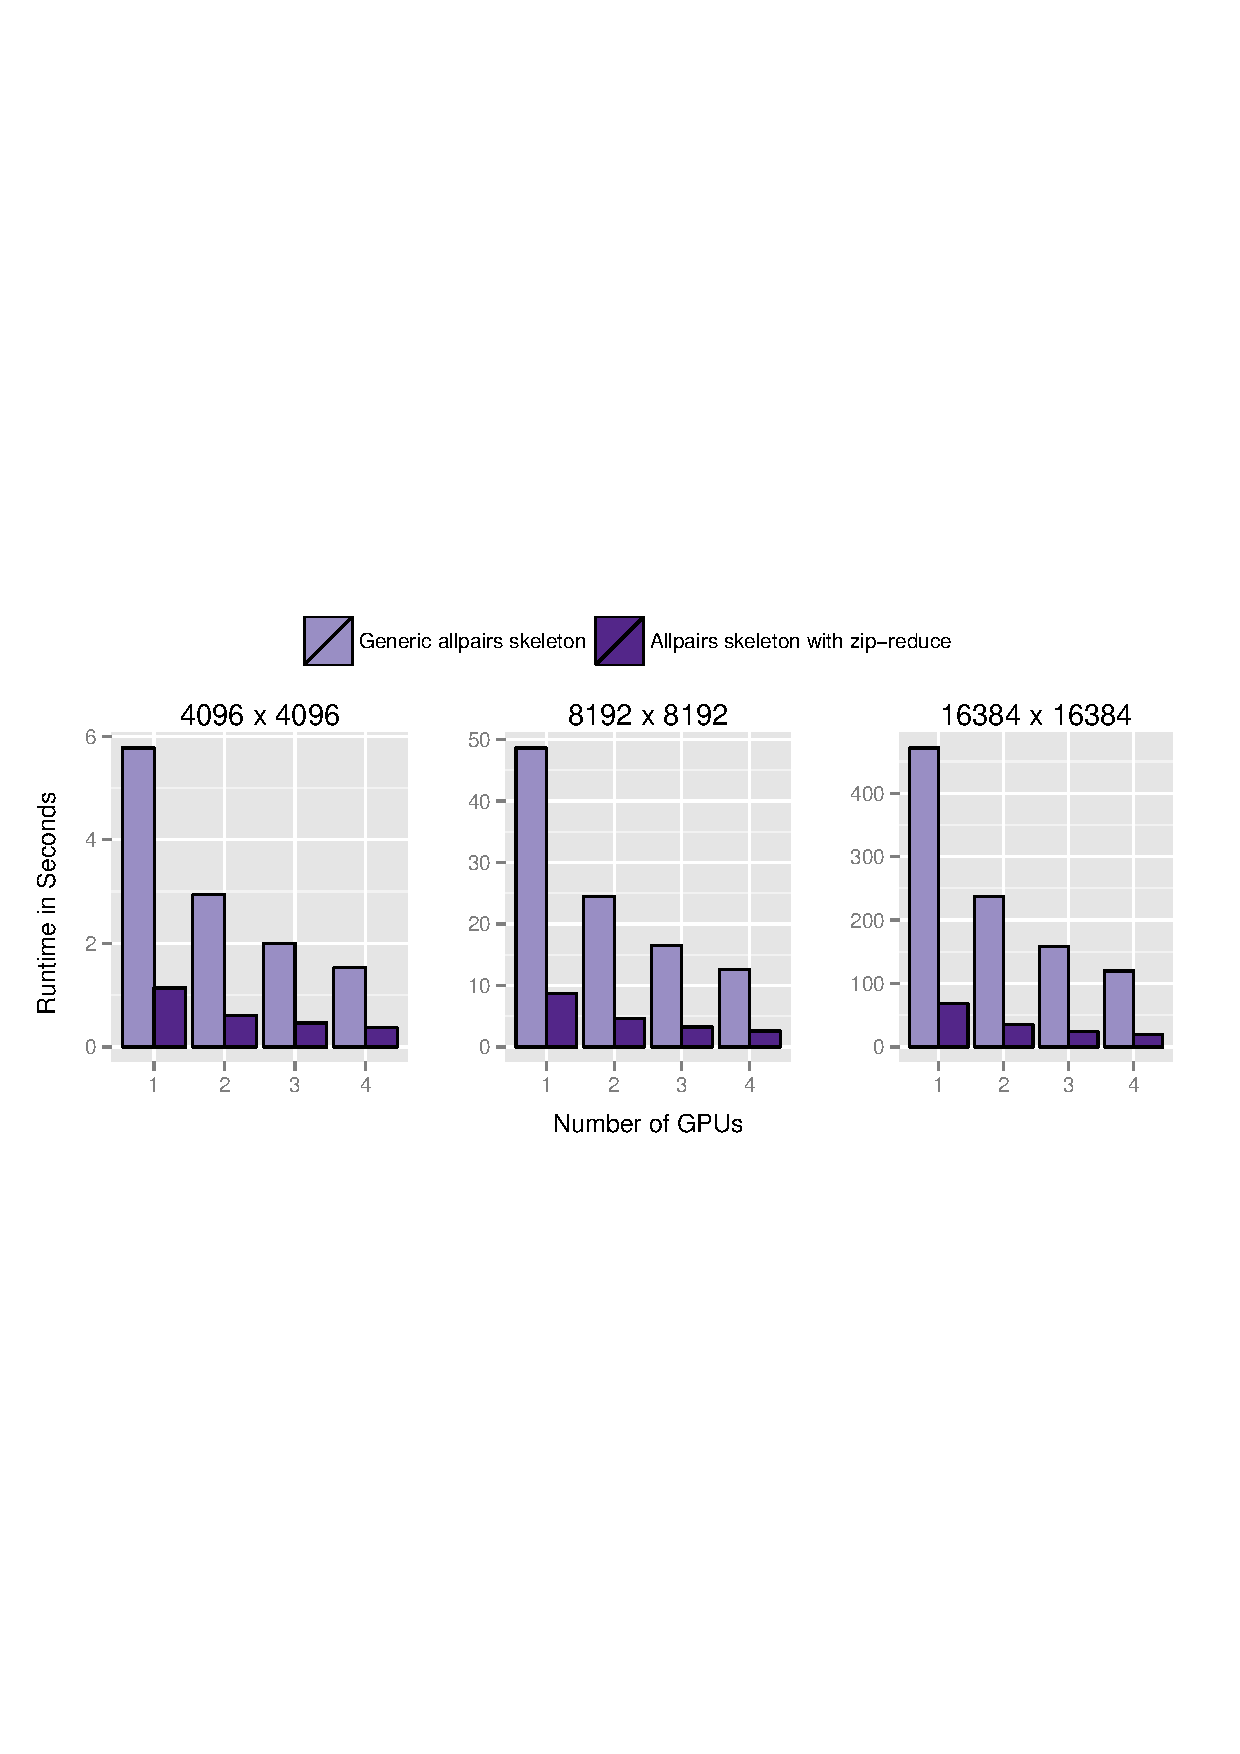
\includegraphics[width=0.9\textwidth]{Plots/MatMult/mat_mult_devices}
  \caption[Runtime of the \allpairs based matrix multiplication implementations using multiple \GPUs]%
          {Runtime of the \allpairs based implementations using multiple \GPUs.}
  \label{fig:mat_mult_devices}
\end{figure}
\begin{table}[tb]
  \centering
  \begin{tabular}{llrrrcr}
    \toprule
              & & \multicolumn{3}{c}{Runtimes in Seconds} & & GFlops\\
    \cmidrule(r){3-5}
    \cmidrule(r){7-7}
    \multirow{2}{*}{Implementation}
     & Number    & $4096$ & $8192$ & $16384$ & & $16384$\\
     & of \GPUs   & $\times 4096$ & $\times 8192$ & $ \times 16384$ & & $ \times 16384$\\
    \midrule
    \multirow{4}{*}{\parbox[t]{2.3cm}{Generic \allpairs\\ skeleton}}
     & 1 \GPU  & 5.772 & 48.645 & 471.328 &&  18.72\\
     & 2 \GPUs & 2.940 & 24.495 & 236.628 &&  37.43\\
     & 3 \GPUs & 2.000 & 16.532 & 158.611 &&  56.17\\
     & 4 \GPUs & 1.527 & 12.540 & 119.786 &&  74.90\\[.5em]
    \multirow{4}{*}{\parbox[t]{2.3cm}{Specialized \allpairs\\ skeleton}}
     & 1 \GPU  & 1.137 &  8.740 &  68.573 && 130.93\\
     & 2 \GPUs & 0.613 &  4.588 &  35.294 && 262.18\\
     & 3 \GPUs & 0.461 &  3.254 &  24.447 && 392.87\\
     & 4 \GPUs & 0.368 &  2.602 &  19.198 && 523.91\\
    \bottomrule
  \end{tabular}
  \caption[Runtime of the \allpairs based implementations of matrix multiplication using multiple \GPUs]%
   {Runtime of the \allpairs based implementations of matrix multiplication using multiple \GPUs.
    For the matrices of size $16384\times 16384$ the results are also shown in GFlops.}
  \label{tab:mat_mult_devices}
\end{table}

\FloatBarrier




\section{Matrix Multiplication}
\label{section:skelcl:matrixMult}

The multiplication of matrices is a fundamental building block for many scientific applications.
A $n\times d$ matrix $A$ is multiplied with a $d\times m$ matrix $B$ to produce a $n\times m$ matrix $C$, where the elements of $C$ are computed as:
\begin{equation*}
  C_{ij} = \sum_{k=0}^{d} A_{ik} \times B_{kj}, \qquad \forall\ i \in 1, \ldots, n \wedge j \in 1, \ldots, m
\end{equation*}
Here $A_{i*}$ refers to the $i$th row of $A$ and $B_{*j}$ to the $j$th column of $B$.
\autoref{fig:mm} visualizes this computation.
To compute the highlighted element in matrix $C$, the highlighted row of matrix $A$ is combined with the highlighted column of matrix $B$.
For computing the entire matrix $C$, \emph{all pairs} of rows from $A$ and columns of $B$ have to be processed.
Therefore, in \SkelCL the \allpairs skeleton can be used to express matrix multiplication.

\begin{figure}[tb]
  \centering
  \includegraphics[width=0.5\textwidth]{HLPP/mm}
  \caption[Visalization of matrix multiplication.]%
          {Matrix multiplication $A\times B = C$.
           The red highlighted element in matrix $C$ is computed by combining the highlighted row of matrix $A$ with the highlighted column of matrix $B$.}
  \label{fig:mm}
\end{figure}


\subsubsection*{\SkelCL Implementation}
\autoref{eq:skelcl:mm} shows how matrix multiplication can be expressed using the \allpairs skeleton in the \SkelCL programming model:
\begin{align}
  \label{eq:skelcl:mm}
  mm\ A\ B &= allpairs\ f\ A\ B^T\\
  \text{where:} \qquad f\ \vec{a}\ \vec{b} &= \sum_{k=0}^d a_k \times b_k \nonumber
\end{align}
When looking back at \autoref{eq:dot_product} in the previous section, we can see, that $f$ is actually the dot product computation, therefore, we can write:
\begin{align}
  mm\ A\ B &= allpairs\ dotProduct\ A\ B^T
  \label{eq:skelcl:mm:dot}
\end{align}
We know that we can express the dot product as a sequential composition of the \zip and \reduce skeletons as we saw in the previous section.
In \autoref{chapter:skelcl}, \autoref{section:skelcl-programming-model:specialSkeletons}, we discussed a specialized implementation of the \allpairs skeleton for computations which can be expressed in this way.
Therefore, we can use the \SkelCL library to develop two implementations:
1) using the generic \allpairs skeleton; and 2) using the specialized \allpairs skeleton.

\autoref{lst:skelcl:mm:generic} shows the implementation of matrix multiplication using the generic \allpairs skeleton.
\begin{lstlisting}[%                                                             
caption={Implementation of matrix multiplication using the generic \allpairs skeleton in \SkelCL.},%
numbers=left,%
float=tb,
label={lst:skelcl:mm:generic}]
Matrix<float> mm(const Matrix<float>& A,$\label{lst:skelcl:mm:generic:CPU:start}$
                 const Matrix<float>& B) {
  skelcl::init();
  auto mm = allpairs($\label{lst:skelcl:mm:generic:CPU:stop}$
    [](const Vector<float>& a, const Vector<float>& b) {$\label{lst:skelcl:mm:generic:GPU:start}$
      float c = 0.0f;
      for (int i = 0; i < a.size(); ++i)
        c += a[i] * b[i];
      return c; });$\label{lst:skelcl:mm:generic:GPU:stop}$
  return mm(A, B); }$\label{lst:skelcl:mm:generic:CPU:call}$
\end{lstlisting}
The skeleton is customized with a lambda expression processing two vectors:
$a$ is a row vector of matrix $A$ and $b$ is a column vector of matrix $B$.
In this generic implementation the dot product computation is implemented using a \code{for} loop iterating over the vectors, multiplying elements pairwise and summing them up in the accumulation variable $c$.

\autoref{lst:skelcl:mm:special} shows the implementation of matrix multiplication using the specialized \allpairs skeleton.
\begin{lstlisting}[%                                                             
caption={Implementation of matrix multiplication using the specialized \allpairs skeleton in \SkelCL.},%
float=tb,%                                                                       
numbers=left,%
label={lst:skelcl:mm:special}]
Matrix<float> mm(const Matrix<float>& A,
                 const Matrix<float>& B) {
  skelcl::init();
  auto mult  = zipVector($\label{lst:skelcl:mm:special:zip}$
      [](float x, float y){return x*y;});$\label{lst:skelcl:mm:special:zipGPU}$
  auto sumUp = reduce($\label{lst:skelcl:mm:special:reduce}$
      [](float x, float y){return x+y;}, 0);$\label{lst:skelcl:mm:special:reduceGPU}$
  auto mm    = allpairs(sumUp, mult);
  return mm(A, B); }
\end{lstlisting}
Here the \allpairs skeleton is customized with \zip and \reduce skeletons defined in \autoref{lst:skelcl:mm:special:zip} and \autoref{lst:skelcl:mm:special:reduce}.
This implementation corresponds more closely to \autoref{eq:skelcl:mm:dot}:
as we express the dot product using these two skeletons (as shown in \autoref{eq:skelcl:dot_product}).
Therefore, we reuse the definitions of \code{mult} and \code{sumUp} as used in \autoref{lst:skelcl:dot}.

\subsubsection*{Implementations used for comparison}
We compare six different implementations of matrix multiplication:
\begin{enumerate}
  \item the \OpenCL implementation from~\cite{KirkHw2010} without optimizations,
  \item the optimized \OpenCL implementation from~\cite{KirkHw2010} using \GPU local memory,
  \item the optimized \BLAS implementation by AMD~\cite{APPML} written in \OpenCL (\clBLAS version 1.10),
  \item the optimized \BLAS implementation by Nvidia~\cite{cuBLAS} written in \CUDA (\CUBLAS version 5.0),
  \item the \SkelCL implementation using the generic \allpairs skeleton shown in \autoref{lst:skelcl:mm:generic},
  \item the \SkelCL implementation using the specialized \allpairs skeleton shown in \autoref{lst:skelcl:mm:special}.
\end{enumerate}

\paragraph{1. OpenCL implementation}
\autoref{lst:naive_opencl} shows the kernel of the first, unoptimized \OpenCL implementation from~\cite{KirkHw2010}.
\begin{lstlisting}[%                                                             
postbreak=\space, breakautoindent=true, breakindent=78pt, breaklines,
caption={[\OpenCL kernel of matrix multiplication without optimizations.]\OpenCL kernel of matrix multiplication without optimizations~\cite{KirkHw2010}.},%
float=tb,%
numbers=left,%
label={lst:naive_opencl}]
kernel void mm(global float* A, global float* B,        global float* C, int m, int d, int n) {
  int row = get_global_id(0);
  int col = get_global_id(1);
  float sum = 0.0f;
  for (int k = 0; k < d; k++)
    sum += A[row * d + k] * B[k * n + col];
  C[row * n + col] = sum; }
\end{lstlisting}

\vspace{-.5em}
\paragraph{2. Optimized OpenCL implementations}
The kernel of the optimized \OpenCL implementation from~\cite{KirkHw2010} using local memory is shown in \autoref{lst:local_mem_opencl}.
\begin{lstlisting}[%                                                             
postbreak=\space, breakautoindent=true, breakindent=78pt, breaklines,
caption={[\OpenCL kernel of the optimized matrix multiplication usgin local memory.]\OpenCL kernel of the optimized matrix multiplication using local memory~\cite{KirkHw2010}.},%
float=tb,%
numbers=left,%
label={lst:local_mem_opencl}]
#define T_WIDTH 16
kernel void mm(global float* A, global float* B,        global float* C, int m, int d, int n) {
  local float Al[T_WIDTH][T_WIDTH];$\label{lst:local_mem_opencl:allocA}$
  local float Bl[T_WIDTH][T_WIDTH];$\label{lst:local_mem_opencl:allocB}$
  int row = get_global_id(0);
  int col = get_global_id(1);
  int l_row = get_local_id(0);
  int l_col = get_local_id(1);
  float sum = 0.0f;
  for (int m = 0; m < d / T_WIDTH; ++m {$\label{lst:local_mem_opencl:loop}$
    Al[l_row][l_col] = A[row * d + (m * T_WIDTH + l_col)];$\label{lst:local_mem_opencl:loadA}$
    Bl[l_row][l_col] = B[(m * T_WIDTH + l_row) * d + col];$\label{lst:local_mem_opencl:loadB}$
    barrier(CLK_LOCAL_MEM_FENCE);$\label{lst:local_mem_opencl:barrier1}$
    for (int k = 0; k < T_WIDTH; k++)
      sum += Al[l_row][k] * Bl[k][l_col];$\label{lst:local_mem_opencl:comp}$
    barrier(CLK_LOCAL_MEM_FENCE); }$\label{lst:local_mem_opencl:barrier2}$
  C[row * n + col] = sum; }
\end{lstlisting}
Two fixed-sized arrays of local memory are allocated in \autoref{lst:local_mem_opencl:allocA} and \autoref{lst:local_mem_opencl:allocB}.
Matrix multiplication is carried out in the loop starting in \autoref{lst:local_mem_opencl:loop}.
In each iteration, data is loaded into the local memory (\autoref{lst:local_mem_opencl:loadA} and \autoref{lst:local_mem_opencl:loadB}) before it is used in the computation in \autoref{lst:local_mem_opencl:comp}.
Note that two synchronization barriers are required (\autoref{lst:local_mem_opencl:barrier1} and \autoref{lst:local_mem_opencl:barrier2}) to ensure that the data is fully loaded into the local memory and that the data is not overwritten while other work-items are still using it.

Both \OpenCL implementations 1. and 2. from~\cite{KirkHw2010} are restrictive:
they are only capable of performing matrix multiplication for square matrices.

\vspace{-.5em}
\paragraph{3. BLAS implementation by AMD}
The implementation offered by AMD is called \clBLAS, written in \OpenCL and is part of their Accelerated Parallel Processing Math Libraries (APPML)~\cite{APPML}.

\vspace{-.5em}
\paragraph{4. BLAS implementation by Nvidia}
\CUBLAS~\cite{cuBLAS} is implemented using \CUDA and, therefore, can only be used on \GPUs built by Nvidia.

\subsubsection*{Programming effort}
\autoref{fig:mat_mult_loc} shows the comparison regarding the number of lines of code (LOCs) required for each of the six implementations.
\autoref{tab:mat_mult_loc} presents the detailed numbers.
We did not count those LOCs which are not relevant for parallelization and are similar in all six implementations, like initializing the input matrices with data and checking the result for correctness.
For every implementation, we distinguish between \CPU (host) code and \GPU (kernel) code.


\begin{figure}[p]
  \begin{minipage}{\textwidth}
  \centering
  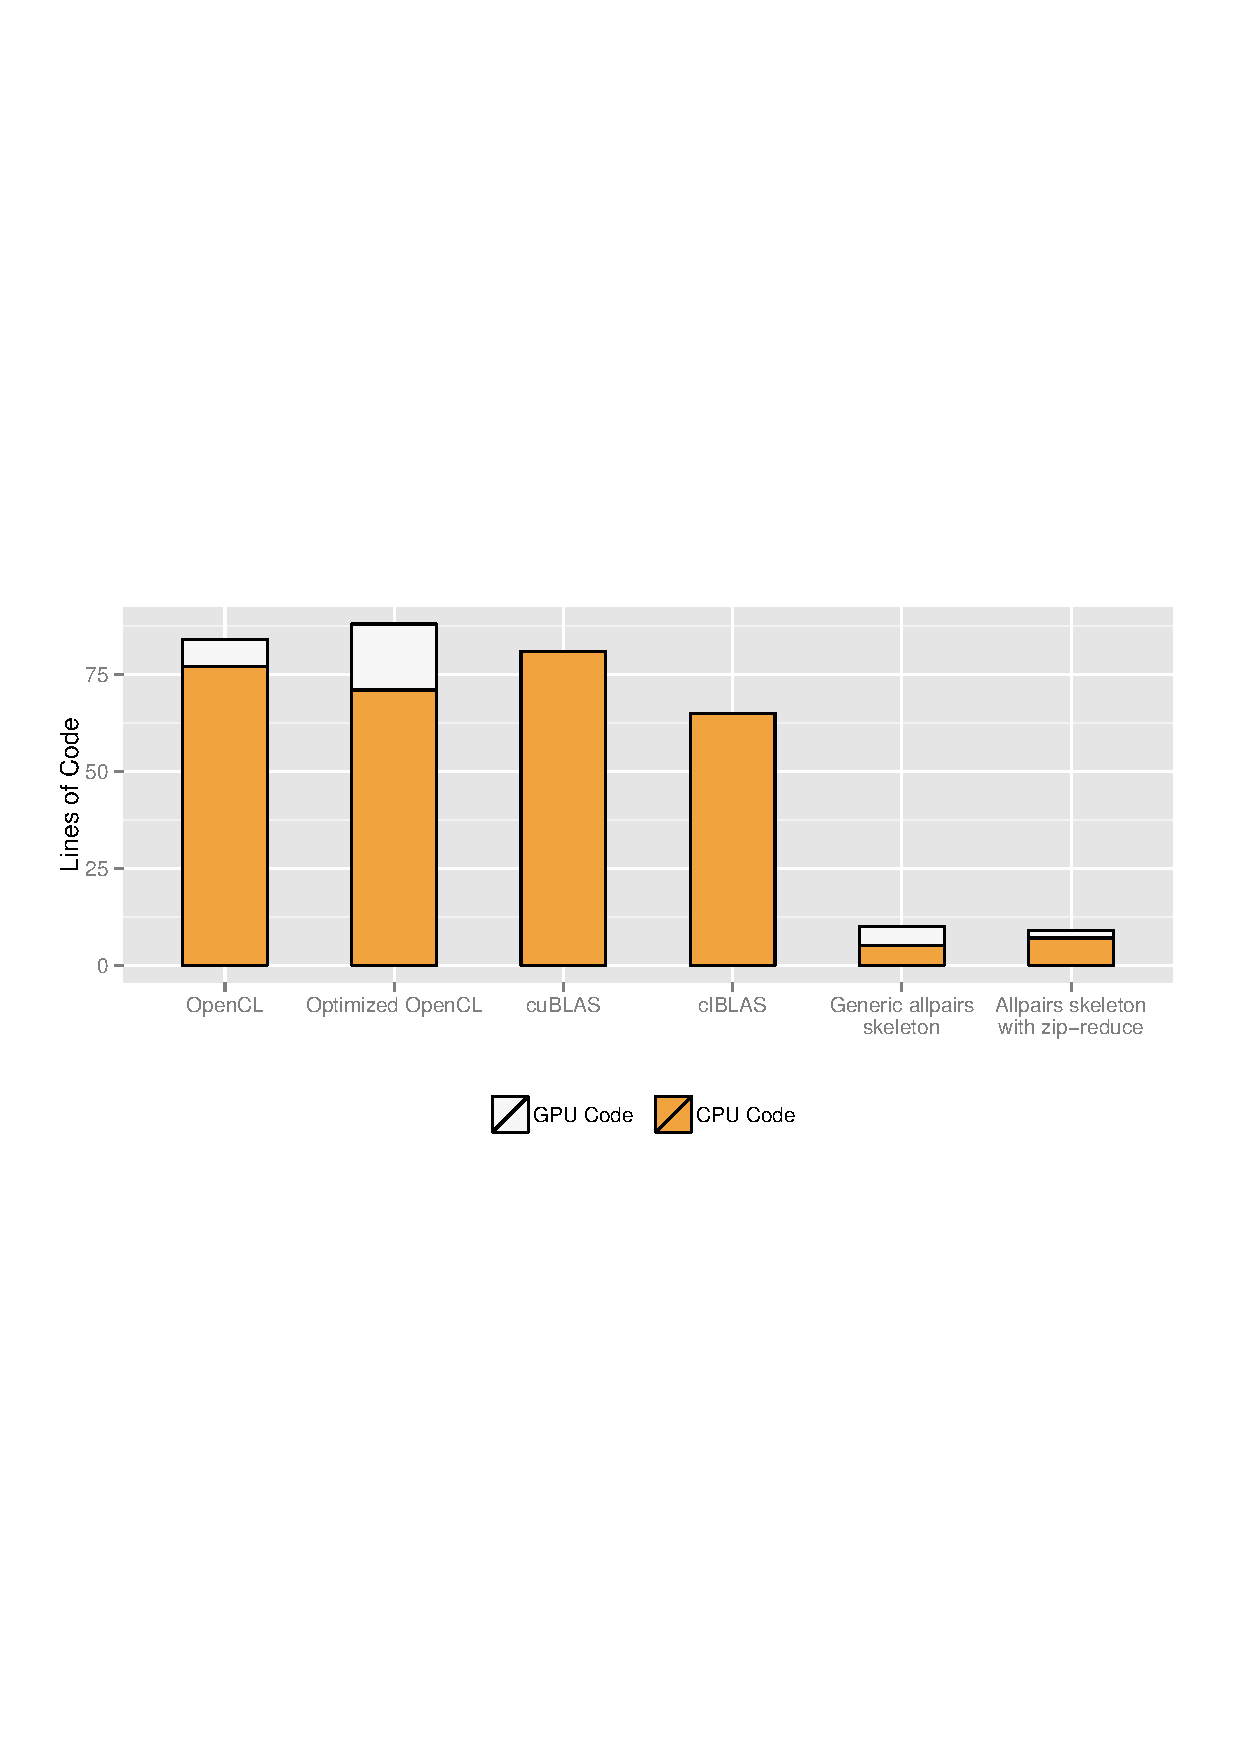
\includegraphics[width=\textwidth]{Plots/MatMult/mat_mult_loc}
  \caption[Programming effort of three \OpenCL-based, one \CUDA-base, and two \SkelCL-based matrix multiplication implementations.]%
          {Programming effort (Lines of Code) of three \OpenCL-based, and one \CUDA-based vs. two \SkelCL-based implementations.}
  \label{fig:mat_mult_loc}
  \end{minipage}
%\end{figure}
%\begin{table}[tb]
\strut\\[2em]\strut
  \begin{minipage}{\textwidth}
  \centering
  \begin{tabular}{lrrr}
    \toprule
              & \multicolumn{3}{c}{Lines of Code} \\
    \cmidrule(r){2-4}
    Implementation & \CPU & \GPU & Total \\[.5em]
    \midrule
    \OpenCL           & 77 &  7 & 84 \\[.5em]
    Optimized \OpenCL & 77 & 17 & 94 \\[.5em]
    \CUBLAS           & 81 & -- & 81\\[.5em]
    \clBLAS           & 65 & -- & 65\\[.5em]
    Generic \allpairs skeleton & 5 & 5 & 10\\[.5em]
    Specialized \allpairs skeleton & 7 & 2 & 9\\[.5em]
    \bottomrule
  \end{tabular}
  \captionof{table}%
          [Lines of Code for matrix multiplication implementaitons.]%
          {Lines of Code of all compared implementations.}
  \label{tab:mat_mult_loc}
  \end{minipage}
%\end{table}
\end{figure}

In the \OpenCL implementations, the \GPU code includes the kernel definition, as shown in \autoref{lst:naive_opencl} and \autoref{lst:local_mem_opencl};
the \CPU code includes the initialization of \OpenCL, memory allocations, explicit data transfer operations, and management of the execution of the kernel.

In the \BLAS implementations, the \CPU code contains the initialization of the corresponding \BLAS library, memory allocations, as well as a library call for performing the matrix multiplication;
no separate definition of \GPU code is necessary, as the \GPU code is defined inside the library function calls.

For the implementation based on the generic \allpairs skeleton (\autoref{lst:skelcl:mm:generic}), we count \autoref{lst:skelcl:mm:generic:CPU:start}---\autoref{lst:skelcl:mm:generic:CPU:stop} and \autoref{lst:skelcl:mm:generic:CPU:call} as the \CPU code, and the definition of the customizing function in \autoref{lst:skelcl:mm:generic:GPU:start}---\autoref{lst:skelcl:mm:generic:GPU:stop} as the \GPU code.
For the implementation based on the specialized \allpairs skeleton (\autoref{lst:skelcl:mm:special}), \autoref{lst:skelcl:mm:special:zipGPU} and \autoref{lst:skelcl:mm:special:reduceGPU} are the \GPU code, while all other lines constitute the \CPU code.

Both skeleton-based implementations are clearly the shortest, with 10 and 9 LOCs.
The next shortest implementation is the \CUBLAS implementation with 65 LOCs -- 7 times longer than the \SkelCL-based implementations.
The other implementations using \OpenCL require even 9 times more LOCs than the \SkelCL-based implementations.

Besides their length, the \OpenCL-based implementations require the application developer to explicitly implement many low-level, error-prone tasks, like dealing with pointers and offset calculations.
Furthermore, the skeleton-based implementations are more general, as they can be used for arbitrary allpairs computations, while all other implementations can compute matrix multiplication only.


\subsubsection*{Performance experiments}
We performed experiments with the six different implementations of matrix multiplication on two different computer systems with \GPUs:
\begin{itemize}[leftmargin=50pt]
  \item[System A:] Our general testing system already described in~\autoref{sec:skelcl:experimental_setup}:
    an Nvidia S1070 equipped with four Nvidia Tesla \GPUs, each with 240 streaming processors and 4 GByte memory.
  \item[System B:] An AMD Radeon HD 6990 card containing two \GPUs, each with 1536 streaming processors and 1 GByte memory.
\end{itemize}

\noindent
We include the data transfer times to and from the \GPU in the results. %, \ie the measured runtime consists of:
% 1) uploading the two input matrices to the \GPU;
% 2) performing the actual matrix multiplication;
% 3) downloading the computed result matrix.


\begin{figure}[tb]
  \centering
  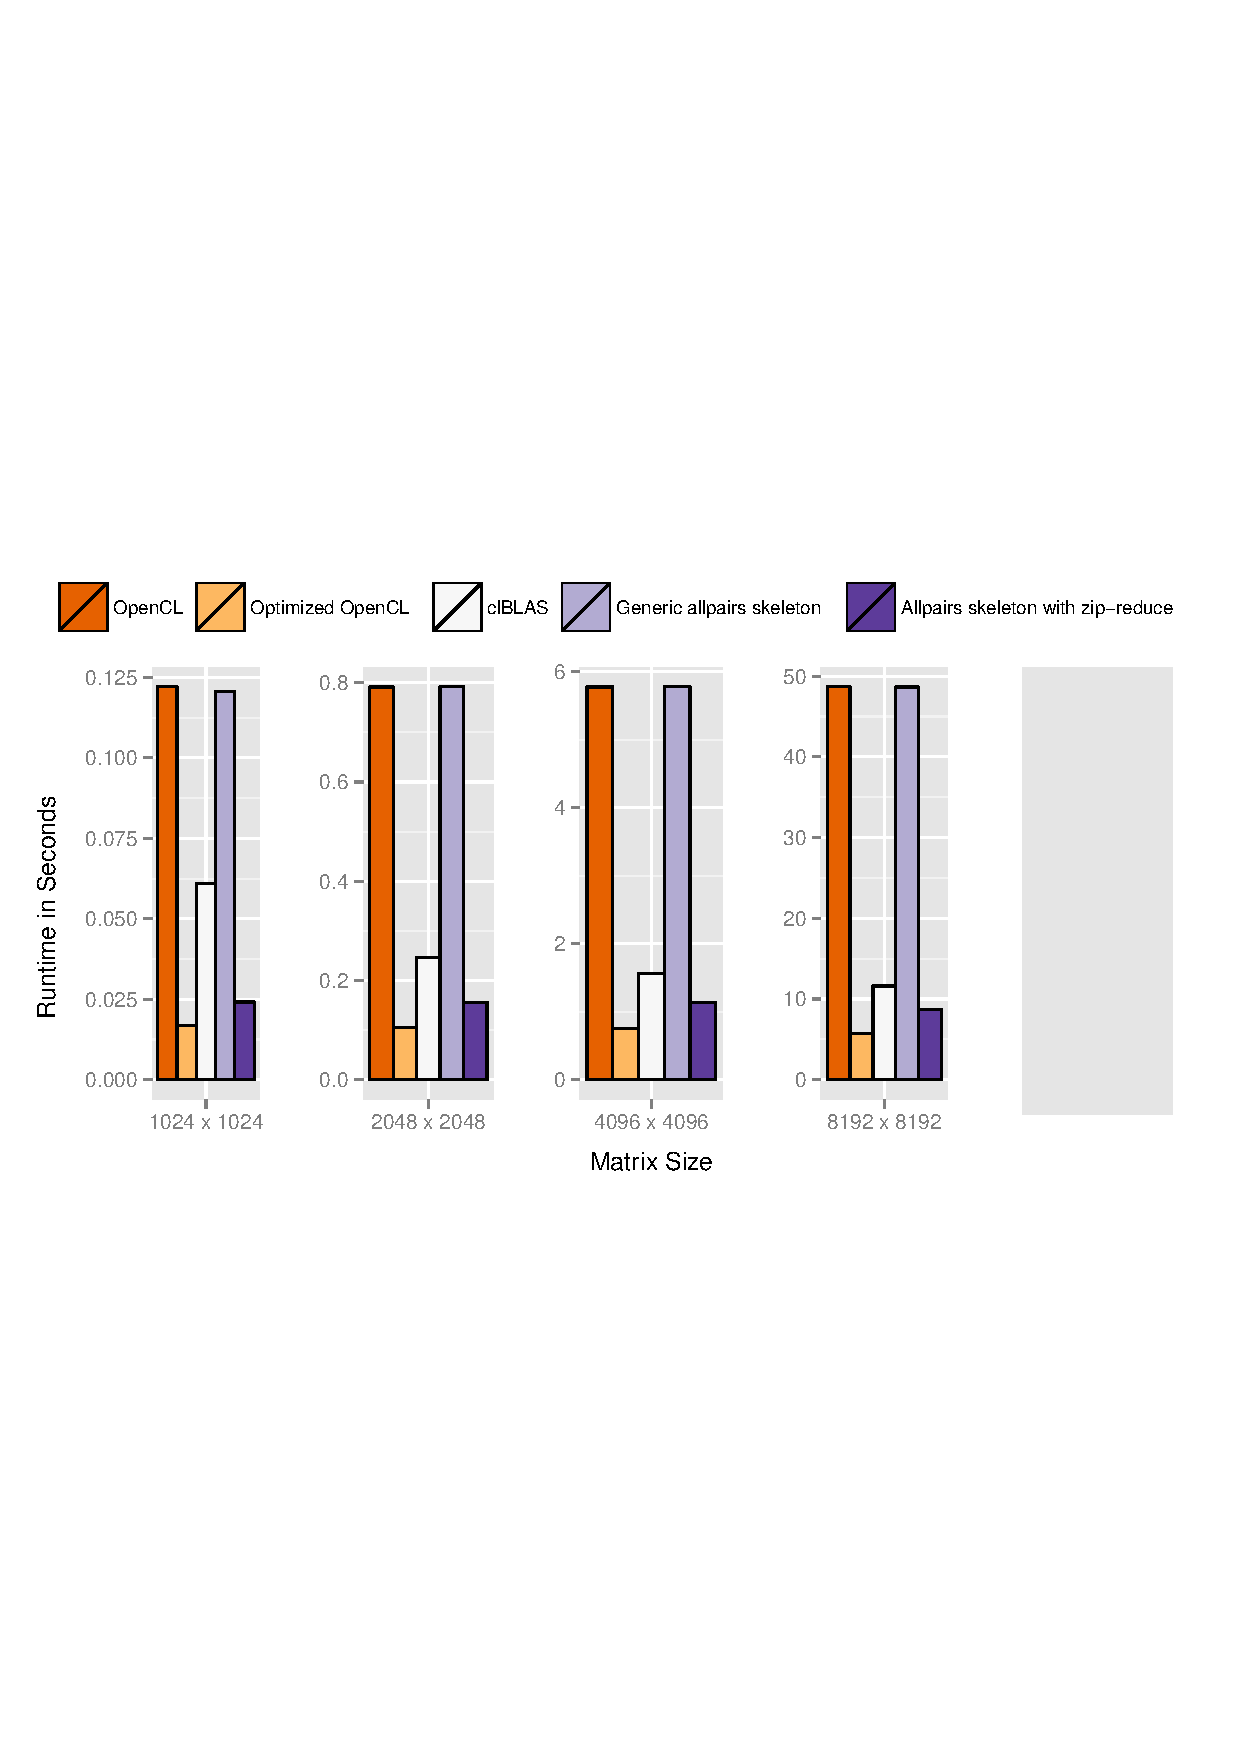
\includegraphics[width=0.8\textwidth]{Plots/MatMult/mat_mult_sizes_gtx480}
  \caption[Runtime of different matrix multiplication implementations on an Nvidia system.]%
          {Runtime of different matrix multiplication implementations on the Nvidia system for different sizes of the matrices.}
  \label{fig:mat_mult_single}
\end{figure}
\begin{table}[tb]
  \centering
  \begin{tabular}{lrrrrr}
    \toprule
              & \multicolumn{5}{c}{Runtimes in Seconds} \\
    \cmidrule(r){2-6}
    \multirow{2}{*}{Implementation} & $1024$ & $2048$ & $4096$ & $8192$ & $16384$ \\
                                    & $\times 1024$ & $\times 2048$ & $\times 4096$ & $\times 8192$ & $\times 16384$\\
    \midrule
    \OpenCL            & 0.122 & 0.791 & 5.778 & 48.682 & 472.557 \\
    Optimized \OpenCL  & 0.017 & 0.105 & 0.752 &  5.683 &  51.337 \\
    \CUBLAS            & 0.012 & 0.059 & 0.387 &  2.863 &  22.067 \\
    \clBLAS            & 0.061 & 0.246 & 1.564 & 11.615 &  90.705 \\
    Generic \allpairs  & \multirow{2}{*}{0.121} & \multirow{2}{*}{0.792} & \multirow{2}{*}{5.782} & \multirow{2}{*}{48.645} & \multirow{2}{*}{471.235} \\[-.5em]
    skeleton\\
    Specialized \allpairs & \multirow{2}{*}{0.024} & \multirow{2}{*}{0.156} & \multirow{2}{*}{1.134} & \multirow{2}{*}{8.742} & \multirow{2}{*}{68.544} \\[-.5em]
    skeleton\\
    \bottomrule
  \end{tabular}
  \caption[Runtime results for matrix multiplication on an Nvidia system.]
          {Runtime results for matrix multiplication on the Nvidia system.}
  \label{tab:mat_mult_single}
\end{table}

\paragraph{System A (one \GPU)}
\autoref{fig:mat_mult_single} shows the runtime of all six implementations for different sizes of the matrices (for readability reasons, all charts are scaled differently).
For detailed numbers, see \autoref{tab:mat_mult_single}.

Clearly, the naive \OpenCL implementation and the implementation using the generic \allpairs skeleton are the slowest, because both do not use local memory, in contrast to all other implementations.

The implementation using the specialized \allpairs skeleton performs 5.0 to 6.8 times faster than the generic allpairs skeleton, but is 33\% slower on the largest matrices than the optimized \OpenCL-based implementation. % using local memory.
However, the latter implementation can only be used for square matrices and, therefore, it benefits from omitting many conditional statements and boundary checks.


\CUBLAS is the fastest of all implementations, as it is highly tuned specifically for Nvidia \GPUs using \CUDA.
The \clBLAS implementation by AMD using \OpenCL performs not as well:
presumably, it is optimized for AMD \GPUs and performs poorly on other hardware.
Our optimized \allpairs skeleton implementation outperforms the \clBLAS implementation for all matrix sizes tested.


\pagebreak

\paragraph{System B (one \GPU)}
\autoref{fig:mat_mult_single_amd} shows the measured runtime in seconds for five of the six implementations for different sizes of the matrices.
Detailed numbers can be found in \autoref{tab:mat_mult_single_amd}.
We could not use the Nvidia-specific \CUBLAS implementation as it does not work on the AMD \GPU.

For bigger matrices, the slowest implementations are, again, the unoptimized \OpenCL implementation and the implementation using the generic \allpairs skeleton.

The optimized \OpenCL implementation and the specialized \allpairs skeleton perform similarly.
For matrices of size $8192\times 8192$, the optimized \OpenCL implementation is about 30\% faster.

The \clBLAS implementation performs very poorly for small matrices, but is clearly the fastest implementation for bigger matrices.
Similar to the \CUBLAS implementation on the Nvidia hardware, it is not surprising that the implementation by AMD performs very well on their own hardware.

\begin{figure}[tb]
  \centering
  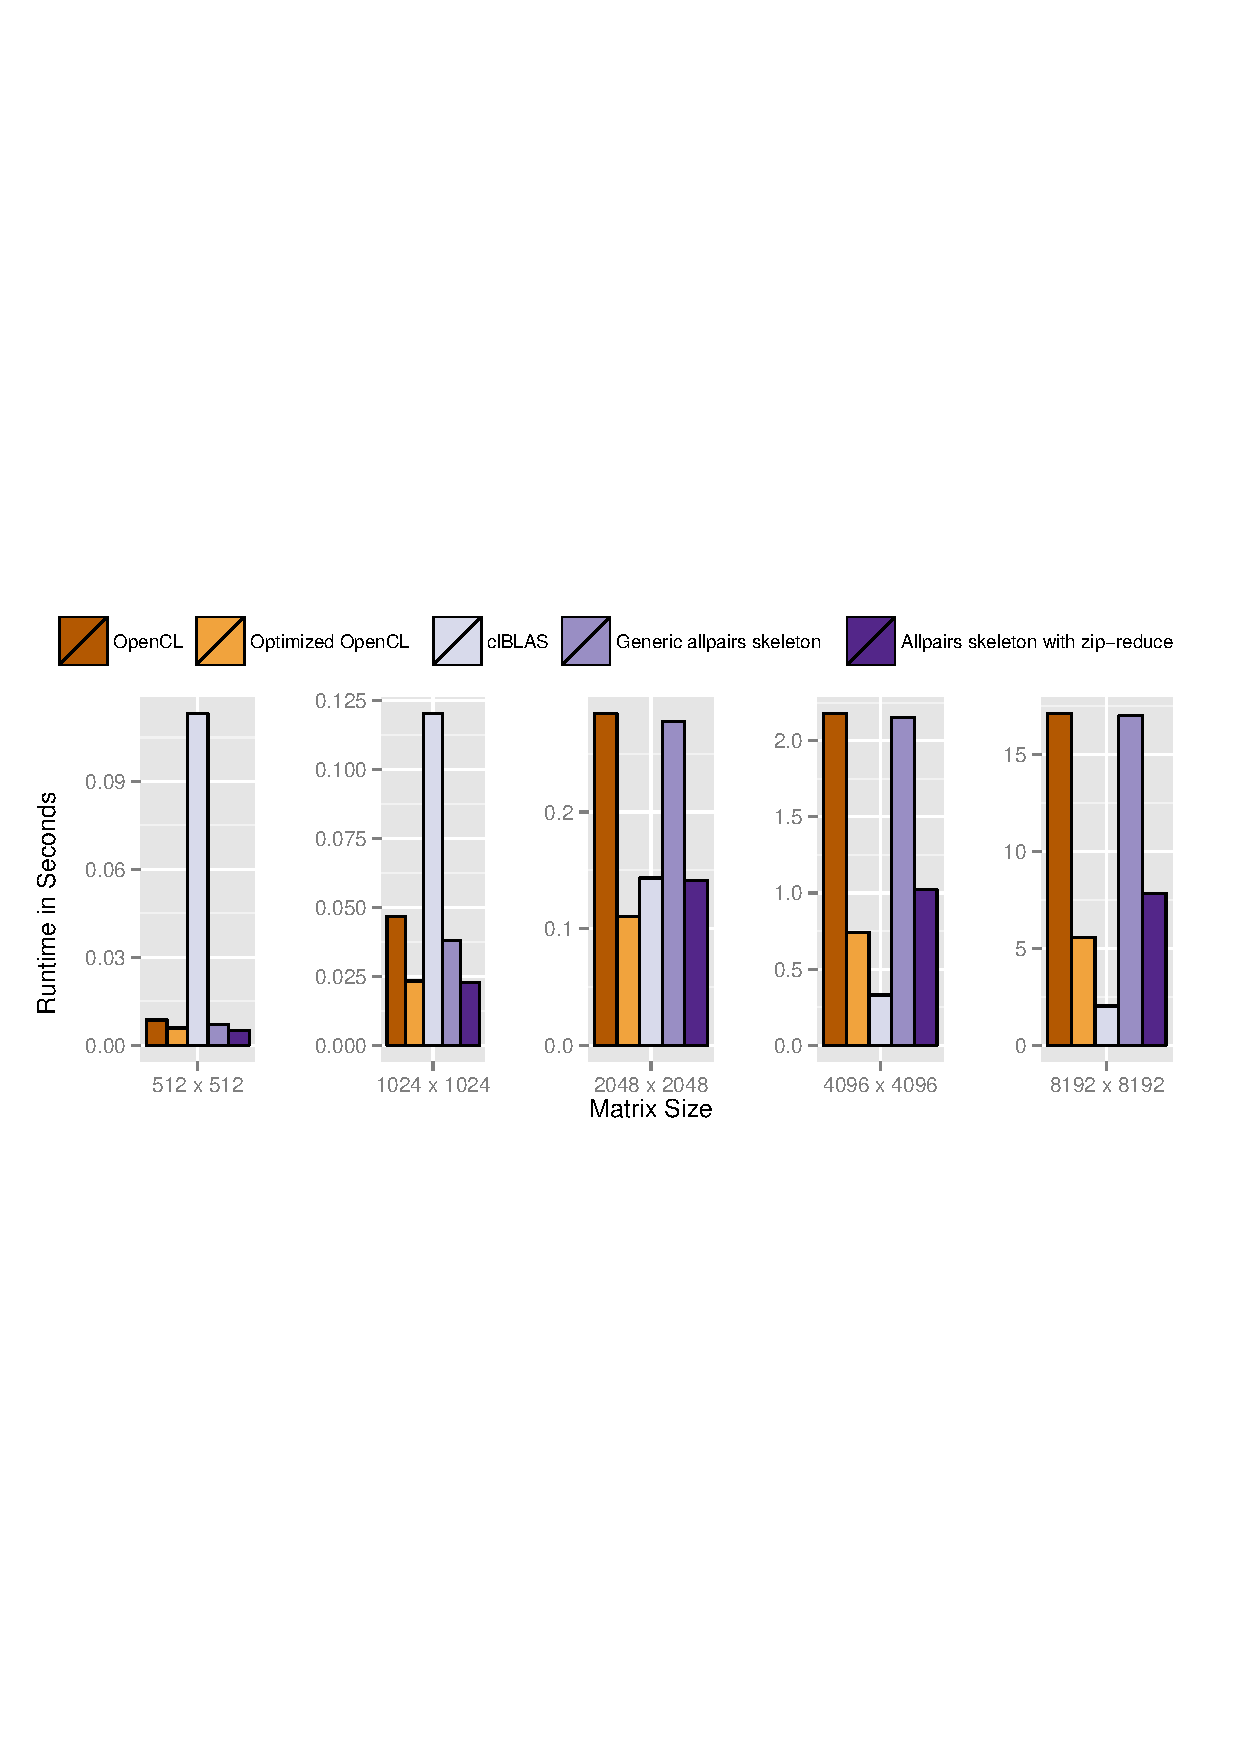
\includegraphics[width=0.8\textwidth]{Plots/MatMult/mat_mult_sizes_hd6990}
  \caption[Runtime of different matrix multiplication implementations on an AMD ststem.]%
          {Runtime of all compared implementations for a matrix multiplication on the AMD system using one \GPU.}
  \label{fig:mat_mult_single_amd}
\end{figure}
\begin{table}[tb]
  \centering
  \begin{tabular}{lrrrrr}
    \toprule
              & \multicolumn{5}{c}{Runtimes in Seconds} \\
    \cmidrule(r){2-6}
    \multirow{2}{*}{Implementation} & $512$ & $1024$ & $2048$ & $4096$ & $8192$ \\
                                    & $\times 512$ & $\times 1024$ & $\times 2048$ & $\times 4096$ & $\times 8192$ \\
    \midrule
    \OpenCL            & 0.008 & 0.046 & 0.284 & 2.178 & 17.098 \\
    Optimized \OpenCL  & 0.006 & 0.023 & 0.111 & 0.743 &  5.569 \\
    \clBLAS            & 0.113 & 0.120 & 0.143 & 0.329 &  2.029 \\
    Generic \allpairs  & \multirow{2}{*}{0.007} & \multirow{2}{*}{0.038} & \multirow{2}{*}{0.278} & \multirow{2}{*}{2.151} & \multirow{2}{*}{16.983} \\[-.5em]
    skeleton\\
    Specialized \allpairs & \multirow{2}{*}{0.005} & \multirow{2}{*}{0.023} & \multirow{2}{*}{0.141} & \multirow{2}{*}{1.025} & \multirow{2}{*}{7.842} \\[-.5em]
    skeleton\\
    \bottomrule
  \end{tabular}
  \caption[Runtime results for all tested implementations of matrix multiplication on an AMD system.]%
          {Runtime results for all tested implementations of matrix multiplication on the AMD system.}
  \label{tab:mat_mult_single_amd}
\end{table}


\pagebreak

\paragraph{System A (multiple \GPUs)}
\autoref{fig:mat_mult_devices} shows the runtime behavior for both \allpairs skeleton-based implementations when using up to four \GPUs of our multi-\GPU system.
The other four implementations are not able to handle multiple \GPUs and would have to be specially rewritten for such systems.
Newer versions of Nvidia's \CUBLAS implementation support the execution on multiple \GPUs as well.
We observe a good scalability for both of our skeleton-based implementations, achieving speedups between 3.09 and 3.93 when using four \GPUs.
Detailed numbers can be found in \autoref{tab:mat_mult_devices}.
For the matrices of size $16384\times 16384$, performance is also provided in GFlops;
to compute this value we excluded the data-transfer time (as usually done in related work) to enable better comparison with related work.

\begin{figure}[tb]
  \centering
  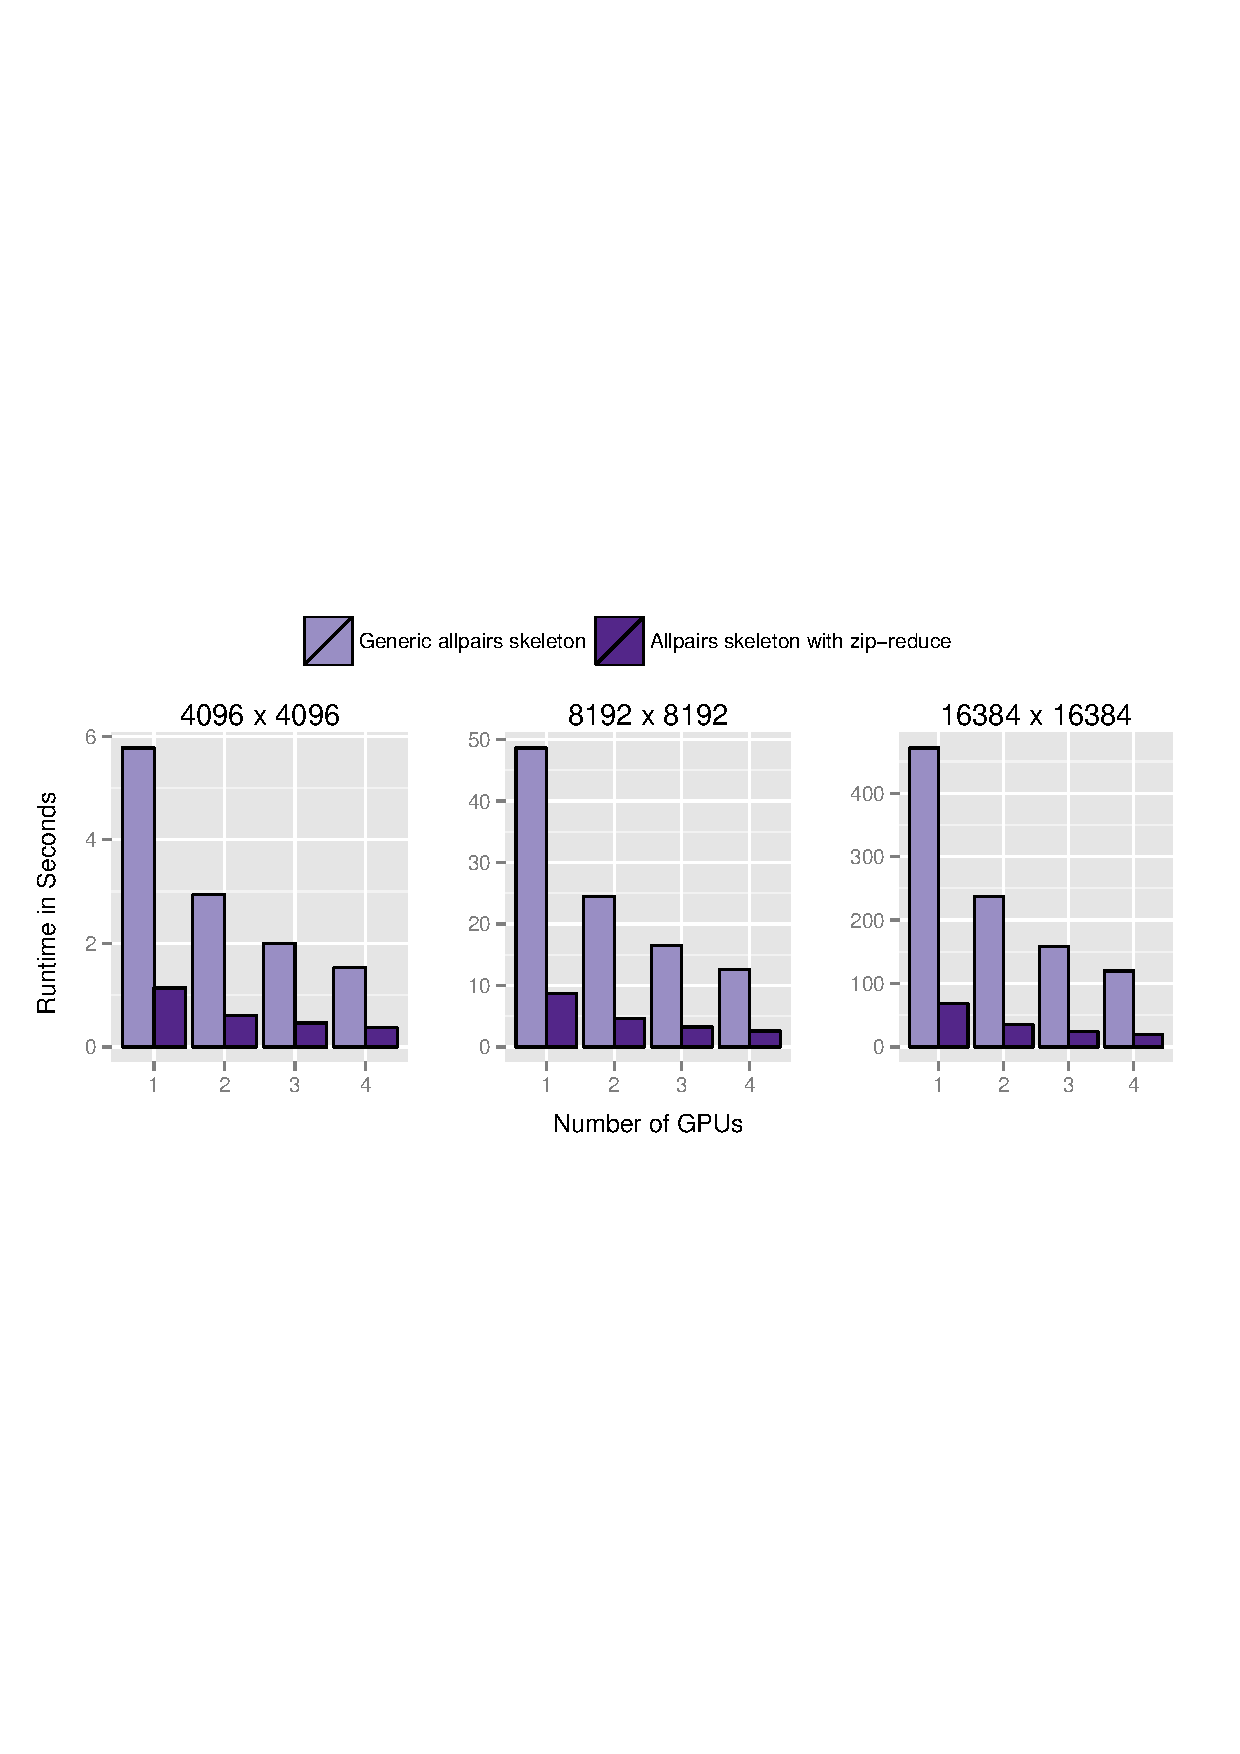
\includegraphics[width=0.9\textwidth]{Plots/MatMult/mat_mult_devices}
  \caption[Runtime of the \allpairs based matrix multiplication implementations using multiple \GPUs]%
          {Runtime of the \allpairs based implementations using multiple \GPUs.}
  \label{fig:mat_mult_devices}
\end{figure}
\begin{table}[tb]
  \centering
  \begin{tabular}{llrrrcr}
    \toprule
              & & \multicolumn{3}{c}{Runtimes in Seconds} & & GFlops\\
    \cmidrule(r){3-5}
    \cmidrule(r){7-7}
    \multirow{2}{*}{Implementation}
     & Number    & $4096$ & $8192$ & $16384$ & & $16384$\\
     & of \GPUs   & $\times 4096$ & $\times 8192$ & $ \times 16384$ & & $ \times 16384$\\
    \midrule
    \multirow{4}{*}{\parbox[t]{2.3cm}{Generic \allpairs\\ skeleton}}
     & 1 \GPU  & 5.772 & 48.645 & 471.328 &&  18.72\\
     & 2 \GPUs & 2.940 & 24.495 & 236.628 &&  37.43\\
     & 3 \GPUs & 2.000 & 16.532 & 158.611 &&  56.17\\
     & 4 \GPUs & 1.527 & 12.540 & 119.786 &&  74.90\\[.5em]
    \multirow{4}{*}{\parbox[t]{2.3cm}{Specialized \allpairs\\ skeleton}}
     & 1 \GPU  & 1.137 &  8.740 &  68.573 && 130.93\\
     & 2 \GPUs & 0.613 &  4.588 &  35.294 && 262.18\\
     & 3 \GPUs & 0.461 &  3.254 &  24.447 && 392.87\\
     & 4 \GPUs & 0.368 &  2.602 &  19.198 && 523.91\\
    \bottomrule
  \end{tabular}
  \caption[Runtime of the \allpairs based implementations of matrix multiplication using multiple \GPUs]%
   {Runtime of the \allpairs based implementations of matrix multiplication using multiple \GPUs.
    For the matrices of size $16384\times 16384$ the results are also shown in GFlops.}
  \label{tab:mat_mult_devices}
\end{table}

\FloatBarrier


\section{Image Processing Applications}
\label{sec:imageProcessing}
Many image processing applications are inherently parallel as they often independently process the pixels of an image.
Common examples range from simple thresholding over noise reduction applications to techniques used in edge detection and pattern recognition~\cite{Umbaugh1997}.
In this section we will study three application examples from image processing and how they can be implemented using \SkelCL.

We start by looking at the Gaussian blur application which can be used to reduce noise in images and is often used as a preprocessing step in more complex algorithms.
We will then discuss two algorithms used for edge detection in images:
the Sobel edge detection application and the more complex Canny edge detection algorithm.

These three applications can all be expressed using the \stencil skeleton introduced in \autoref{section:skelcl-programming-model:specialSkeletons}, but they have different characteristics.
The Gaussian blur applies a single stencil computation, possibly iterated multiple times, for reducing the noise in images.
The Sobel edge detection applies a stencil computation once to detect edges in images.
The more advanced Canny edge detection algorithm consists of a sequence of stencil operations which are applied to obtain the final result.
For each of the three applications, we compare the performance using our two implementations of the \stencil skeleton:
\code{MapOverlap} and \code{Stencil} with native OpenCL implementations using an input image of size $4096 \times 3072$.










\subsection{Gaussian Blur}
\label{sec:gauss}
The Gaussian blur is a standard algorithm used in image processing~\cite{Umbaugh1997}.
One common application is reduction of image noise as shown in \autoref{fig:lena:noise}.
%
\begin{figure}[tb]
  \centering
  \begin{subfigure}[t]{.45\textwidth}
    \includegraphics[width=\textwidth]{lenaNoise2}
    \caption{The Lena image with noise.}
    \label{fig:lena:noise:yes}
  \end{subfigure}
  \hfill
  \begin{subfigure}[t]{.45\textwidth}
    \includegraphics[width=\textwidth]{lenaNoNoise}
    \caption{The Lena image after applying the Gaussian blur.}
    \label{fig:lena:noise:no}
  \end{subfigure}
  \caption{Effect of applying the Gaussian blur to an noised image.}
  \label{fig:lena:noise}
\end{figure}
%
The image on the left has some noise as it is typically produced by halftone printing used to print newspapers.
The Gaussian blur has been applied to reduce the noise and produce the image on the right.

The Gaussian blur computes a weighted average for every pixel based on the neighboring pixels color values.
Using \SkelCL this application can easily be expressed using the \stencil skeleton.

\subsubsection*{\SkelCL Implementation}
\autoref{eq:gauss} shows the Gaussian blur expressed in the \SkelCL programming model using the \stencil skeleton.
\begin{align}
  gauss&\ M = stencil\ f\ 1\ \overline{0}\ M \qquad\text{where:}\nonumber\\
  &
  \begin{array}{ll}%
  f\ &\left[\begin{array}{lll}%
      \hspace{-.5em} M_{i-1,j-1}& \hspace{-.5em} M_{i-1,j} & \hspace{-.5em}M_{i-1,j+1}\vspace{-.25em}\\%
      \hspace{-.5em} M_{i,j-1}& \hspace{-.5em} M_{i,j} & \hspace{-.5em}M_{i,j+1}\vspace{-.25em}\\%
      \hspace{-.5em} M_{i+1,j-1}& \hspace{-.5em} M_{i+1,j} & \hspace{-.5em}M_{i+1,j+1}
    \end{array}\right]  = \\[2em]
          &\qquad \displaystyle\frac{\displaystyle\sum_{k=-1}^{1} \sum_{l=-1}^{1} (G\ k\ l)\cdot M_{i+k, j+k}}{9},
  \end{array} \label{eq:gauss}\\[1em]
  &G\ x\ y = \frac{1}{2\pi \sigma^{2}} e^{-\frac{x^2 + y^2}{2\sigma^2}} \nonumber\\
  \text{and } \overline{0} \text{ is th}&\text{e constant function always returning zero.}\nonumber
\end{align}
The function $G$ is the two-dimensional Gaussian function which is used in the customizing function $f$ to weight the neighboring values $M_{i,j}$.
The values obtained by applying $G$ can be precomputed, as $G$ is only evaluated with values in the interval $[-1, 1]$ for $x$ and $y$.


\autoref{lst:skelcl:gauss} shows the \SkelCL-based implementation of the Gaussian blur using the \code{MapOverlap} implementation of the \stencil skeleton.
Here the immediate neighboring pixels are accessed (lines~\ref{lst:skelcl:gauss:start}--\ref{lst:skelcl:gauss:end}) and used to compute a weighted value for each pixel.
The function computing the weighted sum is omitted here.
It is also possible to extend the \emph{range} of the Gaussian blur and include more neighboring pixel values in the computation.

\begin{lstlisting}[%                                                             
caption={Implementation of the Gaussian blur in \SkelCL using the \code{MapOverlap} implementation of the \stencil skeleton.},%
numbers=left,%
float=tb,
label={lst:skelcl:gauss}]
Matrix<char> gaussianBlur(const Matrix<char>& image) {
  auto gauss = mapOverlap(
    [](Neighborhood<char>& in) {
      char ul = in[{-1, -1}];$\label{lst:skelcl:gauss:start}$
      ...
      char lr = in[{+1, +1}];$\label{lst:skelcl:gauss:end}$
      return computeGaussianBlur(ul, ..., lr); },
    1, BorderHandling::NEUTRAL(0));
  return gauss(image); }
\end{lstlisting}

\subsubsection*{Programming effort}

\begin{figure}[tbp]
	\centering
	\includegraphics[width=\columnwidth]{Plots/gauss/gauss_loc.pdf}
	\caption[Lines of code of the Gaussian blur using different implementations.]%
          {Lines of code of the Gaussian blur using a na{\"i}ve OpenCL implementation with global memory, an optimized OpenCL version using local memory, and \SkelCL's \code{MapOverlap} and \code{Stencil} implementations of the \stencil skeleton.}
	\label{fig:gaussLOCs}
\end{figure} 

\autoref{fig:gaussLOCs} shows the program sizes (in lines of code) for the four implementations of the Gaussian blur. 
The application developer needs $57$ lines of OpenCL host code and 13 LOCs for performing a Gaussian blur only using global memory. 
When using local memory, some more arguments are passed to the kernel, thus, increasing the host-LOCs to $65$, while the LOCs for the kernel function, which copies all necessary elements for a work-group's calculation into local memory, requires $88$ LOCs including explicit out-of-bounds handling and complex index calculations.
The \code{MapOverlap} and \code{Stencil} versions are similar and both require only $15$ LOCs host code and $9$ LOCs kernel code to perform a Gaussian blur. 
The support for multi-\GPU systems is implicitly provided when using \SkelCL's skeletons, such that the kernel remains the same as for one-\GPU systems.
This is an important advantage of \SkelCL over the \OpenCL implementations of the Gaussian blur which are single-\GPU only and require additional LOCs when adapting them for multi-\GPU environments.

\subsubsection*{Performance experiments}

\begin{figure}[tbp]
	\centering
	\includegraphics[width=\columnwidth]{Plots/gauss/gauss_runtime.pdf}
	\caption[Runtime of the Gaussian blur using different implementations.]%
          {Runtime of the Gaussian blur using a na{\"i}ve OpenCL implementation with global memory, an OpenCL version using local memory and SkelCL's MapOverlap and Stencil skeletons.}
	\label{fig:gaussAbs}
\end{figure} 

\autoref{fig:gaussAbs} shows the measured total runtime including data transfers of the Gaussian blur using:
\begin{itemize}
  \item[1)] a na{\"i}ve OpenCL implementation using global memory,
  \item[2)] an optimized OpenCL version using local memory,
  \item[3)] \code{MapOverlap}-based implementation, and
  \item[4)] the \code{Stencil}-based implementation, correspondingly.
\end{itemize}
We can observe that for larger stencil shape sizes, the \code{MapOverlap} and \code{Stencil}-based versions outperform the na{\"i}ve OpenCL implementation by $65\%$ and $62\%$, respectively.
The optimized OpenCL version, which copies all necessary elements into local memory prior to calculation, is $5\%$ faster than \code{MapOverlap} and $10\%$ faster than \code{Stencil} for small stencil shapes.
When increasing the stencil shape size, this disadvantage is reduced to $3\%$ for \code{MapOverlap} and $5\%$ for \code{Stencil} with stencil shape's extent of $10$ in each direction.

The \code{Stencil} implementation is slower for small stencil shapes than the \code{MapOverlap} implementation, up to $32\%$ slower for an stencil shape size of $1$.
This is due to the increased branching required in the \code{Stencil} implementation, as discussed in more detail in \autoref{sec:skelcl:stencil}.
However, this disadvantage is reduced to $4.2\%$ for the stencil shape size of $5$ and becomes negligible for bigger stencil shape sizes.
% Due to the increased branching in Stencil's kernel function, one might expect a worse runtime for the Stencil skeleton. 
As the ratio of copying into local memory decreases in comparison to the number of calculations when enlarging the stencil shape's size, the kernel function's runtime in the \code{Stencil} implementation  converges to the \code{MapOverlap} implementation's time.
The \code{Stencil} implementation's disadvantage is also due to its ability to manage multiple stencil shapes and explicitly support the use of iterations.
While both features are not used in this application example, they incur some overhead for the implementation as compared to the \code{MapOverlap} implementation for simple stencil computations.


\autoref{fig:GaussMult} shows the speedup achieved on the Gaussian blur using the \code{Stencil} implementation on up to four devices.
The higher the computational complexity for increasing size of stencil shape, the better the overhead is hidden, leading to a maximum speedup of $1.90$ for two devices, $2.66$ for three devices, and $3.34$ for four devices, for a size of the stencil shape of 20.
\begin{figure}
	\centering
	\includegraphics[width=.85\columnwidth]{Plots/gauss/gauss_speedup.pdf}
	\caption{Speedup of the Gaussian blur application on up to four \GPUs.}
	\label{fig:GaussMult}
\end{figure} 










\subsection{Sobel Edge Detection}
\label{sec:sobel}
The Sobel edge detection produces an output image in which the detected edges in the input image are marked in white and plain areas are shown in black.
The effect is shown in \autoref{fig:sobel:lena}, where the original image is shown on the left and the output of Sobel edge detection applied to it on the right.

\begin{figure}[tb]
  \centering
  \begin{subfigure}[t]{.45\textwidth}
    \includegraphics[width=\textwidth]{Paraphrase/lena.png}
    \caption{Original image.}
    \label{fig:lena:orig}
  \end{subfigure}
  \hfill
  \begin{subfigure}[t]{.45\textwidth}
    \includegraphics[width=\textwidth]{Paraphrase/sobel_filtered-lena.png}
    \caption{Image after Sobel edge detection.}
    \label{fig:lena:sobel}
  \end{subfigure}
  \caption[The Lena image before and after applying Sobel edge detection.]%
          {The Lena image~\cite{Lena} often used as an example in image processing before (left) and after (right) applying Sobel edge detection.}
  \label{fig:sobel:lena}
\end{figure}

\begin{lstlisting}[%
caption={Sequential implementation of the Sobel edge detection.},%
float=tb,
label={lst:sobel:seq}]
for (i = 0; i < width; ++i)
  for (j = 0; j < height; ++j)
    h = -1*img[i-1][j-1] +1*img[i+1][j-1]
        -2*img[i-1][j  ] +2*img[i+1][j  ]
        -1*img[i-1][j+1] +1*img[i+1][j+1];
    v = ...;
    out_img[i][j] = sqrt(h*h + v*v);
\end{lstlisting}
\bigskip

\autoref{lst:sobel:seq} shows the sequential algorithm of the Sobel edge detection in pseudo-code, with omitted boundary checks for clarity.
In this version, for computing an output value \code{out\_img[i][j]} the input value \code{img[i][j]} and the direct neighboring elements are weighted and summed up horizontally and vertically.
The \stencil skeleton is a perfect fit for implementing the Sobel edge detection.

\subsubsection*{\SkelCL Implementation}
\autoref{eq:sobel} shows the implementation of the Sobel edge detection in the \SkelCL programming model.
\begin{align}
  \label{eq:sobel}
  sobel\ M& = stencil\ f\ 1\ \overline{0}\ M \qquad\text{where:}\\
  f\ &\left[\begin{array}{lll}%
      \hspace{-.5em} M_{i-1,j-1}& \hspace{-.5em} M_{i-1,j} & \hspace{-.5em}M_{i-1,j+1}\vspace{-.25em}\\%
      \hspace{-.5em} M_{i,j-1}& \hspace{-.5em} M_{i,j} & \hspace{-.5em}M_{i,j+1}\vspace{-.25em}\\%
      \hspace{-.5em} M_{i+1,j-1}& \hspace{-.5em} M_{i+1,j} & \hspace{-.5em}M_{i+1,j+1}
    \end{array}\right] = \displaystyle\sqrt{ h^2 + v^2 }\nonumber\\
  h & = \sum_{k=0}^2 \sum_{l=0}^2 Gx_{k, l}\cdot M_{i+k-1,j+k-1}\nonumber\\
  v & = \sum_{k=0}^2 \sum_{l=0}^2 Gy_{k, l}\cdot M_{i+k-1,j+k-1}\nonumber\\
  Gx& = \left[\begin{array}{ccc}%
      -1&0&+1\\
      -2&0&+2\\
      -1&0&+1
    \end{array}\right]
  Gy = \left[\begin{array}{ccc}%
      -1&-2&-1\\
      0&0&0\\
      +1&+2&+1
    \end{array}\right] \nonumber\\
  \text{and } \overline{0} \text{ is th}&\text{e constant function always returning 0.}\nonumber
\end{align}
The formula resembles the sequential implementation shown in \autoref{lst:sobel:seq} where the final result is computed as the square root of the sum of two squared terms $h$ and $v$.
These are computed as weighted sums of the neighboring values $M_{i,j}$.
The weights are given by the two matrices $Gx$ and $Gy$.

\autoref{lst:sobel:skelcl} shows the \SkelCL implementation using the \code{MapOverlap} implementation of the \stencil skeleton.
%
\begin{lstlisting}[%
caption={\SkelCL implementation of the Sobel edge detection.},%
numbers=left,
float=tb,
label={lst:sobel:skelcl}]
Matrix<char> sobelEdge(const Matrix<char>& image) {
  auto sobel = mapOverlap(
    [](Neighborhood<char>& in) {
      short h = -1*in[{-1,-1}] +1*in[{+1,-1}]
                -2*in[{-1, 0}] +2*in[{+1, 0}]
                -1*in[{-1,+1}] +1*in[{+1,+1}];
      short v = ...;
      return sqrt(h*h + v*v); },
    1, BorderHandling::NEUTRAL(0));
  return soble(img); }
\end{lstlisting}
%
The implementation is straightforward and very similar to the formula in \autoref{eq:sobel} and the sequential version in \autoref{lst:sobel:seq}.

\subsubsection*{Programming effort}

\begin{lstlisting}[%
caption={Additional boundary checks and index calculations for Sobel algorithm, necessary in the standard OpenCL implementation.},%
float=tb,
numbers=left,
label={lst:sobel:opencl}]
kernel void sobel_kernel( global const uchar* img,
                          global       uchar* out_img) {
 uint i = get_global_id(0);   uint j = get_global_id(1);
 uint w = get_global_size(0); uint h = get_global_size(1);
 // perform boundary checks
 if(i >= 1 && i < (w-1) && j >= 1 && j < (h-1)) {
  char ul = img[((j-1)*w)+(i-1)];
  char um = img[((j-1)*w)+(i+0)];
  char ur = img[((j-1)*w)+(i+1)];
  // ... 5 more
  char lr = img[((j+1)*w)+(i+1)];

  out_img[j * w + i] = computeSobel(ul, um, ur, ..., lr); }}
\end{lstlisting}

\autoref{lst:sobel:opencl} shows a part of the rather simple \OpenCL implementation for Sobel edge detection provided by AMD as an example application in their software development kit~\cite{AMDSDK}.
The actual computation is performed inside the \texttt{computeSobel} function, which is omitted in the listing, since it is quite similar to the sequential version in \autoref{lst:sobel:seq}.
The listing shows that extra low-level code is necessary to deal with technical details, like boundary checks and index calculations, which are arguably quite complex and error-prone.

We also compare against a more optimized \OpenCL implementation by Nvidia which makes use of the fast local \GPU memory.

The \SkelCL implementation is significantly shorter than the two \OpenCL-based implementations.
The \SkelCL program only comprises few lines of code as shown in \autoref{lst:sobel:skelcl}.
The AMD implementation requires 37 lines of code for its kernel implementation and the more optimized Nvidia implementation requires even 208 lines of code.
Both versions require additional lines of code for the host program which manages the execution of the \OpenCL kernel.
No index calculations or boundary checks are necessary in the \SkelCL version whereas they are crucial for a correct implementation in \OpenCL.

\subsubsection*{Performance experiments}

\begin{figure}[tbp]
  \vspace{.5em}
  \centering
  \includegraphics[height=4.5cm]{Plots/Sobel/sobel_runtime.pdf}
  \caption{Performance results for Sobel edge detection}
  \label{fig:sobel:measurements}
\end{figure}
\autoref{fig:sobel:measurements} shows the measured runtime of the two \OpenCL versions (from the AMD and Nvidia SDKs) vs. the \SkelCL version with the \stencil skeleton presented in \autoref{lst:sobel:skelcl}.
Here only the kernel runtimes are shown, as the data transfer times are equal for all versions.
We used the popular Lena image~\cite{Lena} with a size of $512\times 512$ pixel as an input.
The AMD version is clearly slower than the two other implementations, because it does not use the fast local memory which the Nvidia implementation and the \code{MapOverlap} implementation of the \stencil skeleton of \SkelCL do.
\SkelCL completely hides the memory management details inside its implementation from the application developer.
The Nvidia and \SkelCL implementations perform similarly fast.
In this particular example, \SkelCL even slightly outperforms the implementation by Nvidia.










\subsection{Canny Edge Detection}
The Canny edge detection algorithm is a more complex algorithm to detect edges in images than the Sobel edge detection presented in the previous section.
For the sake of simplicity we consider a slightly simplified version, which applies the following stencil operations in a sequence:
1), a noise reduction operation is applied, \eg, a Gaussian blur;
2), an edge detection operator like the Sobel edge detection is applied;
3), the so-called non-maximum suppression is performed, where all pixels in the image are colored black except pixels being a local maximum;
4), a threshold operation is applied to produce the final result.
A more complex version of the algorithm performs the edge tracking by hysteresis, as an additional step.
This results in detecting some weaker edges, but even without this additional step the algorithm usually achieves good results.


\subsubsection*{\SkelCL Implementation}
In \SkelCL, each single step of the Canny algorithm can be expressed using the \stencil skeleton.
The last step, the threshold operation, does not need access to neighboring elements, as the user threshold function only checks the value of the current pixel.
Therefore, this step can be expressed using \SkelCL's simpler \map skeleton.
In the \SkelCL library the \code{Stencil} skeleton's implementation automatically uses the simpler \map skeleton's implementation when the user specifies a stencil shape which extents are $0$ in all directions.

\begin{lstlisting}[%
  caption={Structure of the Canny algorithm expressed as a sequence of skeletons.},%
  float=tbp,%
  label={lst:skelcl:canny}]
Matrix<char> sobelEdge(const Matrix<char>& image) {
  auto gauss     = stencil(...);$\label{lst:skelcl:canny:step1}$
  auto sobel     = stencil(...);
  auto nms       = stencil(...);
  auto threshold = stencil(...);$\label{lst:skelcl:canny:stepN}$
  StencilSequence<Pixel(Pixel)>
      canny(gauss, sobel, nms, threshold);$\label{lst:skelcl:canny:combine}$
  return canny(image); }$\label{lst:skelcl:canny:call}$
\end{lstlisting}

To implement the Canny algorithm in \SkelCL, the single steps can be combined as shown in \autoref{lst:skelcl:canny}.
The individual steps are defined in lines~\ref{lst:skelcl:canny:step1}--\ref{lst:skelcl:canny:stepN} and then combined to a sequence of stencils in line~\ref{lst:skelcl:canny:combine}.
During execution (line~\ref{lst:skelcl:canny:call}), the stencil operations are performed in the order which is specified when creating the \code{StencilSequence} object.

%\subsubsection*{Programming effort}

\subsubsection*{Performance experiments}

\begin{figure}[tbp]
	\centering
	\includegraphics[width=.75\columnwidth]{Plots/Canny/canny_runtime.pdf}
	\caption[Runtime of the Canny edge detection algorithm.]%
          {Runtime of the Canny edge detection algorithm comparing the \code{MapOverlap} and \code{Stencil} skeleton implementations.}
	\label{fig:canny}
\end{figure} 

\autoref{fig:canny} shows the measured runtime of the Canny algorithm using the two presented implementations.
As the \code{MapOverlap} implementation appends padding elements to the matrix representing the image, the matrix has to be downloaded, resized and uploaded again to the \GPU between every two steps of the sequence.
This additional work leads to an increased time for data transfers. 
The Gaussian blur with a stencil shape extent of $2$, as well as the Sobel edge detection and the non-maximum suppression with a stencil shape of $1$, are $2.1$ to $2.2$ times faster when using \code{MapOverlap}. 
However, the threshold operation, which is expressed as the \map skeleton in the Stencil sequence, is $6.8$ times faster than \code{MapOverlap}'s threshold operation.
Overall, we observe that when performing sequences of stencil operations, the \code{Stencil} implementation reduces the number of copy operations and, therefore, leads to a better overall performance.
When performing the Canny algorithm, the \code{Stencil} implementation outperforms the \code{MapOverlap} implementation by $21\%$.



\section{Medical Imaging}

\from{HIPS begin}
\subsection{List-mode OSEM (HIPS)}

\emph{List-Mode Ordered Subset Expectation Maximization} (list-mode OSEM) is a time-intensive, production-quality algorithm from a real-world application in medical image reconstruction.
It is used to reconstruct three-dimensional images from huge sets of so-called \emph{events} recorded in \emph{positron emission tomography} (PET).
Each event represents a \emph{line of response} (LOR) which intersects the scanned volume.
A simplified sequential implementation of list-mode OSEM is shown in Listing~\ref{lst:lmosem_seq}.
The algorithm splits the events into \emph{subsets} which are processed iteratively:
All LORs of a subset's events and their corresponding intersection \emph{paths} are computed and merged into an \emph{error image} which is merged with the reconstruction image, thus refining a \emph{reconstruction image} in each iteration.

\begin{lstlisting}[%
caption={Sequential implementation of list-mode OSEM.},%
float=bp,%
label={lst:lmosem_seq}]
for	(l = 0; l < num_subsets; l++) {
	/* read subset from file */
	events = read_events();
	/* compute error image c */
	for	(i = 0; i < num_events; i++) {
		/* compute path of LOR */
		path = compute_path(events[i]);
		/* compute error */
		for	(fp = 0, m = 0; m<path_len; m++)
			fp += f[path[m].coord] * path[m].len;
		/* add path to error image */
		for (m = 0; m<path_len; m++)
			c[path[m].coord] += path[m].len / fp;
	}
	/* update reconstruction image f */
	for	(j = 0; j < image_size; j++)
		if (c[j] > 0.0) f[j] *= c[j];	}
\end{lstlisting}

In a parallel implementation of list-mode OSEM, the loops for calculating the error image ($c$) and for updating the reconstruction image ($f$) can be parallelized.

\subsubsection{Programming effort}

We develop implementations of list-mode OSEM using OpenCL and SkelCL; a CUDA-based implementation using multiple GPUs has already been implemented~\cite{ScVG-08}.
Both, CUDA and OpenCL, require us to add a considerable amount of boilerplate code for running a kernel on multiple GPUs, in particular for uploading and downloading data to and from the GPUs.
In CUDA, we have to create one CPU thread for each device to be managed.
This introduces the additional challenge of multi-threaded programming, including the need of thread synchronization.

\begin{lstlisting}[%
caption={Implementation of list-mode OSEM in SkelCL.},%
float=tbp,%
label={lst:lmosem_skelcl}]
for (l = 0; l < num_subsets; l++) {
	// read events from file
	Vector<Event> events(read_events());
	
	// distribute events to devices
	events.setDistribution(
		Distribution::block);
	// copy reconstruction (f) and error image (c) to all devices
	f.setDistribution(Distribution::copy);
	c.setDistribution(Distribution::copy);
	
	// prepare arguments of error image computation
	SkelCL::Arguments arguments;
	arguments.push(events);
	arguments.push(events.size());
	arguments.push(paths); // memory for paths
	arguments.push(f);
	arguments.push(c);
	
	// compute error image (map skeleton)
	compute_c(index, arguments);
	
	// signal modification of error image
	c.dataOnDevicesModified();
	// distribute reconstruction image to  all devices
	f.setDistribution(Distribution::block);
	// reduce (element-wise add) all copies of error image; re-distribute to all devices after reduction
	c.setDistribution(Distribution::block, add);
	
	// update reconstruction image (zip skeleton)
	update(f, c, f);	}
\end{lstlisting}

With SkelCL, we use the \texttt{Vector} class and the \texttt{Map} and \texttt{Zip} skeletons to implement list-mode OSEM (see Listing~\ref{lst:lmosem_skelcl}).
The events of a subset, as well as the error image and the reconstruction image are stored in a SkelCL \texttt{Vector}.
Thus, we can easily distribute subsets across all GPUs and copy both images to all devices.
We use a \texttt{Map} skeleton to implement the computation of the error image.
However, we must not compute too many paths in parallel to avoid excessive memory consumption.
Therefore, the input of the \texttt{Map} skeleton is not a subset, but rather a vector of 512 indices.
These indices refer to disjoint sub-subsets of events, each of which is processed within a single kernel instance on the GPUs.
For each event, this kernel performs the same steps as the first inner loop in the sequential implementation.
The reconstruction and the error image, as well as the events, are passed to the \texttt{Map} skeleton as additional arguments.
The skeleton produces no result, but updates the error image by side-effect.
Therefore, the error image has to be marked as ``modified on the device'' after executing the \texttt{Map} skeleton.

So far, separate copies of the error image have been used on all GPUs.
To obtain the final error image, we have to merge all copies into a single image.
Afterwards, the final error image and the reconstruction image are distributed across all GPUs, such that each device processes a part of these images.
In SkelCL, the aforementioned data movement is easily achieved by changing the kind of distribution of the vectors that contain this data.
A \texttt{Zip} skeleton is used to implement the update of the reconstruction image, taking the distributed images as input.
The kernel function of this skeleton resembles the body of the second inner loop of the sequential implementation.

The parallelization using SkelCL is quite similar to our CUDA- and OpenCL-based implementations.
However, when using SkelCL's vector data type, we avoid additional programming effort to implement data transfer between host and GPU or between multiple GPUs, and we obtain a multi-GPU-ready implementation of list-mode OSEM for free.
The SkelCL-based implementation is the shortest with 232 lines of code (kernel function: 200~lines, host program: 32~lines).
The CUDA- and OpenCL-based implementations are considerably longer with 329 (199, 130), or even 436 lines of code (193, 243), respectively (see Figure~\ref{fig:lmosem_results}).


\subsubsection{Performance experiments}

We tested our implementations of list-mode OSEM using a typical data set of about $10^7$ events for $150\times 150\times 280$ PET image.
The data set is split into 10 equally sized subsets.
We measured the average runtime of processing all subsets.
Figure~\ref{fig:lmosem_results} shows the runtime of our three implementations of list-mode OSEM using one, two, and four GPUs.

\begin{figure}[tbp]
	\centering
	\label{fig:lmosem_runtime}%
	\label{fig:lmosem_speedup}%
	\includegraphics[width=0.42\textwidth]{HIPS/ChartLmosem}
	\caption{Runtime and program size of parallel list-mode OSEM using CUDA, OpenCL, and SkelCL.}
	\label{fig:lmosem_results}
\end{figure}

Running on a single GPU, the CUDA-based implementation (3.03 seconds) outperforms the ones based on OpenCL and SkelCL (3.66 seconds each) by about 20\%.
These relative performane differences also hold for using two GPUs, with only negligible overhead of SkelCL compared to OpenCL.
With four GPUs, the CUDA-based implementation again is faster than the SkelCL- (23\%) and OpenCL-based (17\%) implementations.
SkelCL provides a speedup of 3.1, while OpenCL and CUDA provide speedups of 3.24 and 3.15 respectively.
On four GPUs the SkelCL code runs 2.56 times faster than the CUDA on one GPU.

The SkelCL-based implementation only introduces a moderate overhead of less than 5\% as compared to OpenCL.
Since the OpenCL-based implementation requires a lot of low-level boilerplate code (over 100 lines of code only for initialization), the SkelCL-based implementation clearly provides a higher level of programming.
Especially, the additional argument feature and the data distributions are crucial for this application as it cannot be implemented efficiently without these two features.
In conclusion, this example shows that SkelCL is suitable for implementing a real-world application and provides performance close to a native OpenCL implementation.
\from{HIPS end}

\from{ASHES begin}
\subsection{Application Study: List-mode OSEM (ASHES)}

To demonstrate the advantages of SkelCL as compared to the contemporary GPU programming models, we implemented a real-world application from the field of medical imaging using SkelCL, OpenCL, and CUDA.
In this section, we compare these three implementations regarding: 1)~programming effort, and 2)~runtime performance.

\emph{List-Mode Ordered Subset Expectation Maximization} (list-mode OSEM)~\cite{Reader98,KSW-11} is a time-intensive, production-quality numerical algorithm for \emph{Positron Emission Tomography} (PET):
it reconstructs three-dimensional images from huge sets of so-called \emph{events} recorded by a tomograph.
Each event recorded represents a \emph{Line Of Response} (LOR) which intersects the scanned volume.

A simplified sequential code of list-mode OSEM is shown in Listing~\ref{lst:list-mode_OSEM:sequential}.
The algorithm splits the events into \emph{subsets} which are processed iteratively:
all LORs of subset events and their corresponding intersection \emph{paths} are computed and merged into an \emph{error image}.
The {error image} is merged with the initially empty \emph{reconstruction image}, which is then refined in each iteration.
In the following, we refer to the computation of the error image as step~1 (lines 5 to 13), and the update of the reconstruction image as step~2 (lines 15 and 16) of the algorithm.

\begin{lstlisting}[%
caption={Simplified sequential code of list-mode OSEM.},%
float,%
label={lst:list-mode_OSEM:sequential},%
numbers=left,%
xleftmargin=2em]
for (l = 0; l < num_subsets; ++l) {
  /* read subset from file */
  events = read_events();
  /* compute error image c (step 1) */
  for (i = 0; i < num_events; ++i) {
    /* compute path of LOR */
    path = compute_path(events[i]);
    /* compute error */
    for (fp = 0, m = 0; m<path_len; ++m)
      fp += f[path[m].coord] * path[m].len;
      /* add path to error image */
      for (m = 0; m<path_len; ++m)
        c[path[m].coord] += path[m].len / fp;
  }
  /* update reconstruction image f (step 2) */
  for (j = 0; j < image_size; ++j)
    if (c[j] > 0.0) f[j] *= c[j];
}
\end{lstlisting}

\begin{figure*}[tbp]
 \centering
 \includegraphics[width=.6\textwidth]{ASHES/lmosem_distribution}
 \caption{Data distribution changes and computations during a single subset iteration of list-mode OSEM using two GPUs.}
 \label{fig:list-mode_OSEM:gpu}
\end{figure*}

\subsubsection{Parallelization strategy}
\label{sec:list-mode_OSEM:strategy}

For parallelization, we consider two possible decomposition strategies for the OSEM algorithm as initially suggested in~\cite{JJK03}: Projection Space Decomposition (PSD) and Image Space Decomposition (ISD).

In PSD, the subsets are split into sub-subsets that are processed simultaneously while all processing units access a common reconstruction and error image.
Using this approach, we are able to parallelize step~1 of the algorithm, but step~2 is performed by a single processing unit.
On a multi-GPU system, we have to copy the reconstruction image to all GPUs before each iteration, and we have to merge all GPUs' error images computed in step~1 before proceeding with step~2.
While both steps are easy to implement, step~2 does not efficiently use the available processing units.

In ISD, the reconstruction image is partitioned, such that each processing unit processes the whole subset with respect to a single part of the reconstruction image.
Thus we are able to parallelize both steps of list-mode OSEM, but each processing unit still accesses the whole reconstruction image in order to compute the error value for each path before merging it with the error image.
On a multi-GPU system, the whole subset has to be copied to each GPU in step~1.
ISD requires large amounts of memory (up to several GB in practically relevant cases) to save all paths computed in step~1.
Summarizing, it is hard to implement step~1 on the GPU, while step~2 can be parallelized easily.

Therefore, we decided to use a hybrid strategy for implementing list-mode OSEM on a multi-GPU system:
Step~1 is parallelized using the PSD approach, while we use ISD for step 2.
This results in the sequence of five phases shown both in Figure~\ref{fig:list-mode_OSEM:gpu} and Listing~\ref{lst:list-mode_OSEM:skelcl}:
\begin{enumerate}
\item \emph{Upload:} the subset ($s$) is divided into sub-subsets, one sub-subset per GPU.
      One sub-subset and the reconstruction image ($f$) are uploaded to each GPU.
\item \emph{Step 1:} each GPU computes a local error image ($c$) for its sub-subset using a map skeleton with additional arguments.
\item \emph{Redistribution:} the local error images that are distributed on all GPUs are downloaded and combined into a single error image on the host by performing element-wise addition.
      Afterwards, the combined error image and reconstruction image are partitioned, in order to switch the parallelization strategy from PSD to ISD.
      The corresponding parts of both images are distributed to the GPUs again.
\item \emph{Step 2:} each GPU updates its part of the reconstruction image using a zip skeleton
\item \emph{Download:} finally, all parts of the reconstruction image are downloaded from the GPUs to the host and merged into a single reconstruction image.
\end{enumerate}

\begin{lstlisting}[%
caption={Parallel implementation of list-mode OSEM in SkelCL.},%
float,%
label={lst:list-mode_OSEM:skelcl},%
numbers=left,%
xleftmargin=2em]
for (l = 0; l < num_subsets; l++) {
  /* 1. Upload: distribute events to devices*/
  Vector<Event> events(read_events());
  events.setDistribution(Distribution::block);
  f.setDistribution(Distribution::copy);
  c.setDistribution(Distribution::copy(add));
  /* 2. Step 1: compute error image
        (map skeleton) */
  mapComputeC(index,events,events.sizes(),f,c);
  c.dataOnDevicesModified();
  /* 3. Redistribution: distribute
        reconstruction image to devices; reduce
        (element-wise add) all error images and
        distribute result to devices */
  f.setDistribution(Distribution::block);
  c.setDistribution(Distribution::block);
  /* 4. Step 2: update reconstruction image
        (zip skeleton) */
  zipUpdate(f, c, f);
  /* 5. Download: merge reconstruction image
        (is performed implicitly) */ }
\end{lstlisting}

The SkelCL program in Listing~\ref{lst:list-mode_OSEM:skelcl} reflects the described five phases in a concise, high-level manner, as shown by the corresponding comments.
The subset, the error image, and the reconstruction image are declared as SkelCL vectors which enables an easy and automatic data transfer between GPUs.
As data transfers are performed implicitly by SkelCL, the upload phase (1.) is implemented by simply setting vector distributions (lines 4--6), while the download phase (5.) is omitted entirely.

\subsubsection{Programming effort: SkelCL vs. OpenCL \& CUDA}
\label{sec:list-mode_OSEM:implementation}

Using the described hybrid parallelization strategy, we developed three parallel implementations of list-mode OSEM using: 1) CUDA, 2) OpenCL, and 3) SkelCL. %~\cite{ScVGM-08}
To study the programming effort, we compare the program sizes in LOC (lines of code).
Though LOC is not a universal measure for programming effort, we consider it as a reasonable first approximation.

We observe~(see Figure~\ref{fig:list-mode_OSEM:LOC}) that while the kernel size in CUDA and OpenCL, or the user-defined function in SkelCL, respectively, are rather similar (about 200 LOC), the lengths of the corresponding host programs differ considerably.
Unlike CUDA, OpenCL requires code for selecting the target platform and an OpenCL device and for compiling kernel functions at runtime.
For a single GPU, the OpenCL-based implementation has the longest code (206 LOC), i.\,e. about 2.5 times longer than the CUDA-based host program (88 LOC) and more than 11 times longer than the SkelCL program.
Our SkelCL-based implementation has 18 LOC, i.\,e. its length is only about 20\% of the CUDA-based version.

Using multiple GPUs in OpenCL and CUDA requires explicit code for additional data transfers between GPUs.
Prior to CUDA 4.0, also multi-threaded code was required to manage several GPUs.
This accounts for additional 42 LOC for the CUDA-based implementation and additional 37 LOC for the OpenCL-based one.
In SkelCL, only 8 additional LOC are necessary to describe the changes of data distribution.
These lines are easily recognizable in the SkelCL program (lines 4--6, 11--12 in Listing~\ref{lst:list-mode_OSEM:skelcl}, plus 3 lines during the initialization) and make this high-level code arguably better understandable and maintainable than the CUDA and OpenCL versions.

\subsubsection{Performance experiments: SkelCL vs. OpenCL \& CUDA}
\label{sec:list-mode_OSEM:runtime}

We evaluated the runtimes of our three implementations of list-mode OSEM, by reconstructing an image of $150\times 150\times 280$ voxels from a real-world PET data set with about $10^8$ events.
From this data set, about $10^2$ equally sized subsets are created.
In our experiments, we measured the average runtime of processing one subset.
In a full reconstruction application, all subsets are processed multiple times, thus making list-mode OSEM a time-intensive application that runs several hours on a single-core CPU.
Unlike CUDA, both OpenCL and SkelCL compile kernels at runtime.
As compilation is only required once, when launching the implementation, but not during the subset iterations, we excluded compilation time from our runtime measurements.
We ran our implementations on a system comprising a quad-core CPU (Intel Xeon E5520, 2.26\,GHz) and an NVIDIA Tesla S1070 system with 4~Tesla GPUs.
Each GPU consists of 240 streaming processors. % running at up to 1.44\,GHz.
The CPU has 12\,GB of main memory, while each GPU owns 4\,GB of dedicated memory.

Figure~\ref{fig:list-mode_OSEM:runtime} shows the runtime of our three implementations of list-mode OSEM using up to four GPUs.
We observe that CUDA always provides best performance, being about 20\% faster than OpenCL and SkelCL on the same number of GPUs.
As compared to the OpenCL-based implementation, SkelCL introduces only a moderate overhead of less than 5\%.
Hence, the runtime overhead of SkelCL as compared to CUDA is mainly caused by the fact that SkelCL is built on top of OpenCL.

\begin{figure}[tb]
  \centering
  \begin{subfigure}{.45\textwidth}
    \includegraphics[width=\textwidth]{ASHES/loc}
    \caption{Lines of code for host (light gray) and GPU (dark gray)}
    \label{fig:list-mode_OSEM:LOC}
  \end{subfigure}
  \hfill
  \begin{subfigure}{.45\textwidth}
    \includegraphics[width=\textwidth]{ASHES/lmosemIteration}
    \caption{Average runtime of one subset iteration}
    \label{fig:list-mode_OSEM:runtime}
  \end{subfigure}
  \caption{Program size of parallel list-mode OSEM (single- and multi-GPU versions), and runtime for processing one subset using SkelCL, OpenCL, and CUDA.}
  \label{fig:list-mode_OSEM:results}
  \bigskip
\end{figure}
\from{ASHES end}

\from{ICCS begin}
\subsection{Iterative PET Image Reconstruction and the LM OSEM Algorithm (ICCS)}
\label{sec:pet}
Our running application example in this paper is the LM OSEM algorithm~\cite{READER, sgmkswb09} for image reconstruction used in Positron Emission Tomography (PET).
In PET, a radioactive substance is injected into a human or animal body, which is then placed inside a PET scanner that contains several arrays of detectors.
As the particles of the applied substance decay, positrons are emitted (hence the name PET) and annihilate with nearby electrons, such that two photons are emitted in the opposite directions (see Fig.~\ref{fig:scanner and detector}).
These ``decay events'' are registered by two opposite detectors of the scanner which records these events in a list.
Data collected by the PET scanner are then processed by a reconstruction algorithm to obtain a resulting image.

\begin{figure}
\centering
\includegraphics[scale=0.50]{ICCS/ringscanner}
\caption{Two detectors register an event in a PET-scanner}
\label{fig:scanner and detector}
\end{figure}

\subsubsection{The LM OSEM Algorithm}
List-Mode Ordered Subset Expectation Maximization \cite{READER} (called LM OSEM in the sequel) is a block-iterative algorithm for 3D image reconstruction.
LM OSEM takes a set of events from a PET scanner and splits them into $s$ equally sized subsets.
Then, for each subset $S_l, l \in {0, \ldots, s-1}$, the following computation is performed:
\begin{equation}
f_{l+1}=f_{l}c_{l};\quad
c_{l}=\dfrac{1}{A_N^T \textbf{1}}
\sum_{i \in S_{l}} (A_i)^T \dfrac{1}{A_{i} f_{l}}.
\label{equ:lm_osem}
\end{equation}

Here $f \in \mathbb{R}^n$ is a 3D image in vector form with dimensions $n = (X \times Y \times Z)$, $A$ -- the so called system matrix, element $a_{ik}$ of row $A_i$ is the length of intersection of the line between the two detectors of event $i$ with voxel $k$ of the reconstruction image, computed with Siddon's algorithm \cite{SIDDON}.
$\dfrac{1}{A_N^T \textbf{1}}$ is the so-called normalization vector; since it can be precomputed, we will omit it in the following.
The multiplication $f_{l}c_{l}$ is performed element-wise.
Each subset's computation takes its predecessor's output image as input and produces a new, more precise image.

The structure of a sequential LM OSEM implementation is shown in Listing~\ref{lst:seq_code}.
The outermost loop iterates over the subsets.
The first inner loop (step 1) iterates over subset's events to compute $c_l$, which requires three sub-steps:
row $A_i$ is computed from the current event using Siddon's algorithm;
the local error for row $A_i$ is computed and, finally, added to $c_l$.
The second inner loop (step 2) iterates over all elements of $f_l$ and $c_l$ to compute $f_{l+1}$.
\begin{figure}
\begin{lstlisting}[caption={Sequential code for LM OSEM comprises one outer loop with two nested inner loops.},label={lst:seq_code}]
for (int l = 0; l < subsets; l++) {
  /* read subset */

  /* step 1: compute error image c_l */
  for (int i = 0; i < subset_size; i++) {
    /* compute A_i            */
    /* compute local error    */
    /* add local error to c_l */  }

  /* step 2: update image estimate f */
  for (int k = 0 ; k < image_size; k++) {
    if (c_l[k] > 0.0) { f[k] = f[k] * c_l[k]; } }  }
\end{lstlisting}
\end{figure}

\subsubsection{Parallelization of LM OSEM in OpenCL}
\label{sec:parallel_implementation}
LM OSEM is a rather time-consuming algorithm that needs parallelization:
a typical 3D image reconstruction processing $6 \cdot 10^7$ input events for a $150 \times 150 \times 280$ PET image takes more than two hours on a modern PC.

Although the iterations of the outer loop in Listing~\ref{lst:seq_code} are inherently sequential,
we can parallelize the two calculation steps within one iteration as shown in Fig.~\ref{fig:em_distribution} for a system comprising one CPU and two GPUs.
Note that these steps require different data distribution patterns:
\begin{itemize}
  \item[] \emph{Step 1:} Subset's events are copied from the CPU to all GPUs (\emph{upload}) to compute the summation part of $c_l$ concurrently. This step requires that the complete image estimate $f_l$ is available to all GPUs.
  \item[] \emph{Step 2:} For computing the next image estimate $f_{l+1}$ in parallel, the current image estimate $f_l$ and the error image $c_l$ computed in step 1 have to be distributed in disjoint parts (blocks) among all GPUs.
\end{itemize}
\begin{figure}
\centering
\includegraphics[width=0.6\textwidth]{ICCS/em_distribution}
\caption{Parallelization schema of the LM OSEM algorithm.}
\label{fig:em_distribution}
\end{figure}
Thus, the parallelization schema in Fig.~\ref{fig:em_distribution} requires a data \emph{redistribution} phase between the two computation steps.
During step 1, each GPU computes a partial sum of $c_l$.
After step 1, all partial results are summed up and redistributed disjointly to all GPUs.
Note that for step 1, each GPU requires a full copy of the image estimate, while in step 2 all GPUs update disjoint parts of it.
After step 2, the disjoint parts of the image estimate are copied from all GPUs back to the CPU (\emph{download}).

\bigskip\noindent
In the following, we describe how the parallelization schema phases in Fig.~\ref{fig:em_distribution} are implemented using OpenCL.

\paragraph{Upload}
The simplified OpenCL implementation of the upload phase is shown in Listing~\ref{lst:upload}.
Uploading of the event vector $S$ is performed in lines 3--6, while lines 9--12 show the upload of the image estimate $f_l$.
In OpenCL, we have to manage each GPU explicitly, therefore, for each GPU, we create a set of buffers (\texttt{s\_gpu} and \texttt{f\_gpu}) and we use a loop (line 1) to repeat all memory operations for each GPU.
For performance reasons, we use asynchronous copy operations, specified using the \texttt{CL\_FALSE} flag (line 3 and 9): this allows data transfers to multiple GPUs to overlap.
We perform different operations with $S$ (distribute among all GPUs) and $f_l$ (copy to each GPU), therefore, there are differences when specifying the amount of bytes to copy (lines 4 and 10) and the offsets in the CPU memory (lines 5 and 11).
Altogether eleven such memory operations -- each with different amounts and offsets -- appear in the OpenCL source code.

\begin{lstlisting}[caption={Implementation of the upload phase in OpenCL (ommitting error checks for brevity)},label={lst:upload},numbers=left]
for (int gpu = 0; gpu < gpu_count; gpu++) {
  // upload $S$
  clEnqueueWriteBuffer( command_queue[gpu], s_gpu[gpu], CL_FALSE, 0,
                        sizeof(float) * size_of_s / gpu_count,
                        (void*)&s_cpu[ gpu * size_of_s / gpu_count ],
                        0, NULL, NULL );

  // upload $f_l$
  clEnqueueWriteBuffer( command_queue[gpu], f_gpu[gpu], CL_FALSE, 0,
                        sizeof(float) * size_of_f,
                        (void*)&f_cpu[0],
                        0, NULL, NULL ); }
\end{lstlisting}

\paragraph{Step 1}
The implementation of step 1 performs the operations shown in Listing~\ref{lst:seq_code}: first computing $A_i$, then the local error for $A_i$ and finally adding the local error to $c_l$.
Because of GPU memory restrictions, the OpenCL implementation is not straightforward, such that, for the sake of brevity, we will not discuss it in more detail here.

\paragraph{Redistribution}
Listing~\ref{lst:redistribution} shows an OpenCL pseudocode for the redistribution phase.
To download the data from all GPUs, we use the \texttt{clEnqueueReadBuffer} function and perform the operations asynchronously, but this time, we have to wait for the operations to finish.
For such synchronization, OpenCL uses \emph{events}, associated with an operation (line 3) for waiting for the operation to finish (line 4).
After all downloads have finished, we combine the different values of $c_l$ to a new value of $c_l$ on the CPU (line 7), and upload the blocks of $c_l$ to the GPUs.
Even if we only copied data between GPUs, without processing them on the CPU, we still would have to download them to the CPU because direct GPU-to-GPU transfers are currently not possible in OpenCL.

\begin{lstlisting}[caption={OpenCL pseudocode for the redistribution phase},label={lst:redistribution},numbers=left]
// download all c_l values from the GPUs to the CPU
cl_event events[gpu_count];
for (int gpu = 0; gpu < gpu_count; gpu++) { clEnqueueReadBuffer( ..., &events[gpu] ); }
clWaitForEvents(gpu_count, events);

// combine data on CPU
combine( ... );

// upload block of the new c_l version to each GPU
for (int gpu = 0; gpu < gpu_count; gpu++) { clEnqueueWriteBuffer( ... ); }
\end{lstlisting}

\paragraph{Step 2}
Listing~\ref{lst:step_2} shows the implementation of step 2.
In OpenCL, computations are specified as \emph{kernels} which are created from the source code specifying the computation.
The computation in step 2 is, therefore, described as a string in lines 3 -- 5.
The operations used here are the same as in the sequential code in Listing~\ref{lst:seq_code}.

For executing the computations of step 2, we have to perform the following steps for each GPU:
\begin{itemize}
  \item create an OpenCL kernel from the source code (requires 50 lines of code in OpenCL);
  \item compile the kernel specifically for the GPU (requires 13 lines of code in OpenCL);
  \item specify kernel arguments one-by-one using the \texttt{clSetKernelArg} function (line 12 -- 17);
  \item specify execution environment, i.\,e., how many instances of the kernel to start (line 20 -- 21);
  \item launch the kernel (line 23 -- 24).
\end{itemize}
\begin{lstlisting}[caption={Implementation of step 2 in OpenCL (omitting error checks for brevity)},numbers=left,label={lst:step_2}]
// step 2 (in Fig. 2)
source_code_step_2 =
"__kernel void step2(__global float* f, __global float* c_l, int offset, int size) { \
  int id = get_global_id(0) + offset;                                                \
  if (id < size && c_l[id] > 0.0) { f[id] = f[id] * c_l[id]; } }";

for (int gpu = 0; gpu < gpu_count; gpu++) {
 // create kernel (50 lines of code)
 // compile kernel (13 lines of code)

 // specifying kernel arguments:
  clSetKernelArg(kernel_step2[gpu], 0, sizeof(cl_mem), (void*)&f_buffer[gpu]);
  clSetKernelArg(kernel_step2[gpu], 1, sizeof(cl_mem), (void*)&c_l_buffer[gpu]);
  int offset = gpu * (size_of_f / gpu_count);
  clSetKernelArg(kernel_step2[gpu], 2, sizeof(int), (void*)&offset);
  int size   = MIN( (gpu + 1) * (size_of_f / gpu_count), size_of_f );
  clSetKernelArg(kernel_step2[gpu], 3, sizeof(int), (void*)&size);

 // specify execution environment
  int local_work_size[1]  = { 32 };
  int global_work_size[1] = { roundUp(32, size_of_f / gpu_count) };
 // launch the kernel
  clEnqueueNDRangeKernel(command_queue[gpu], kernel_step2[gpu],
                         1, NULL, &global_work_size, &local_work_size, 0, NULL, NULL); }
\end{lstlisting}


\paragraph{Download}
The implementation of the download phase is similar to the upload phase (Listing~\ref{lst:upload}).
\from{ICCS end}

\from{ICCS begin}
\subsection{Implementing the LM OSEM Algorithm using SkelCL (ICCS)}
\label{sec:experiments}
\label{sec:experiments:skelcl}
We assess the programming effort and runtime performance of our approach by comparing the SkelCL implementation of the LM OSEM algorithm against its OpenCL implementation.

\paragraph{Programming effort}

The parallel SkelCL code in Listing~\ref{lst:em_skelcl} fully retains the original sequential structure of Listing~\ref{lst:seq_code}, which makes it well structured and easily understandable.
\begin{lstlisting}[%
  caption={SkelCL code of the LM OSEM algorithm},%
  numbers=left,%
float,%
label={lst:em_skelcl}]
Map<void(int)> computeC_l("void func(int index, event* s, float* f, float* c_l) {   \
  for (int i = index; i < subset_size; i+=512) {                                    \
    // compute A_i // compute local error // add local error to c_l                 \
  } }");
Zip<float(float, float)> updateF("float func(float f_i, float cl_i) {               \
      if (cl_i > 0.0) return f_i * cl_i; else return f_i; }");

Vector<float> f   = readStartImage();
Vector<int> index = createIndexVector(512);
for (i = 0; i < num_iterations; ++i) {
  Vector<event> s = read_subset(); // read subset s from file
  Vector<float> c_l(image_size);
  s.setDistribution(block);
  f.setDistribution(copy);
  c_l.setDistribution(copy, add);

  /* step 1. compute error image c_l */
  computeC_l(index, s, f, c_l);

  f.setDistribution(block);
  c_l.setDistribution(block);

  /* step 2. update image estimate f */
  f = updateF(f, c_l); }
\end{lstlisting}
The sequential loops are replaced by skeleton calls (line 18 and 24) which take the code from the corresponding loop's body, and only 5 lines of code are added for data distribution (lines 13 -- 15 and 20 -- 21).
The computation of the error image is expressed using a map skeleton (lines 1 -- 4).
Due to memory restrictions, it is not possible to apply the map skeleton to the whole vector \texttt{s}:
map is rather applied to a vector of size 512 (line 9), such that for every index a block of elements is processed using the loop in line 2.
Since detecting memory restrictions and applying blocking automatically is non-trivial, SkelCL currently relies on the user to resolve such situations.
The event vector, the image estimate, and the error image are passed as additional arguments to the skeleton.
The zip skeleton is used for updating the error image (line 5 -- 6).

The SkelCL-based implementation of the LM OSEM is considerably shorter than the OpenCL code:
with 232 lines of code (customizing functions: 200~lines, host program: 32~lines) as compared to 436 lines of code (kernel functions: 193~lines, host program: 243~lines) in the OpenCL-based implementation; we save almost 50\% of the lines of code.
When using SkelCL, we do not have to implement the tedious and lengthy initialization of OpenCL.
Expressing the computations as skeletons liberates us from dealing with pointers in the kernel and repeatedly performing the same sequence of steps for each computation.
By using container data types, we avoid additional programming effort to implement data transfers between CPU and GPU or between multiple GPUs, and we obtain a multi-GPU-ready implementation of LM OSEM for free.


\paragraph{Runtime performance}
We tested the performance of our implementations using an NVIDIA Tesla S1070 system comprising 4 Tesla GPUs.
Each GPU consists of 240 streaming processors.

Fig.~\ref{fig:lmosem_runtime} compares the runtime of one iteration for our SkelCL and OpenCL implementations using one, two, and four GPUs, correspondingly.
While the differences in the programming effort to implement the two versions are significant, the differences in runtime are very small.
When running on a single GPU, both implementations take the same time (3.66 seconds) to complete.
With two and four GPUs, the OpenCL implementation slightly outperforms the SkelCL implementation, being 1.2\% and 4.7\% faster.
We presume that the increasing overhead is caused by the more complex data distribution performed when using more GPUs.
Comparing to the significant reduction in programming effort (50\%), the runtime overhead of less than 5\% is arguably a moderate one.
\vfill
\begin{figure}
  \centering
  \includegraphics[width=.4\textwidth]{ICCS/skelcl-runtime.pdf}
  \caption{Average runtime of one iteration of the LM OSEM algorithm using SkelCL and OpenCL.}
  \label{fig:lmosem_runtime}
\end{figure}
\from{ICCS end}



\section{Physics Simulation}
\label{sec:physicsSim}

Physics simulations are a very important class of scientific applications.
We study one representative: the \emph{Finite-Difference-Time-Domain (\FDTD) Method} used for Random Lasing Simulations.
This simulation from the field of optical physics simulates the propagation of light through a medium.

In the simulation two fields, the electric field $\vec{E}$ and the magnetic field $\vec{H}$, are iteratively updated using stencil computations.
We use the Maxwell's equations which are the basic equations describing electrodynamic processes in nature to describe the light propagating through a non-magnetic (\emph{dielectric}) medium.

\autoref{eq:div_e}---\autoref{eq:rot_d} show the Maxwell's equations consisting of four coupled partial differential equations (PDEs).
\begin{align}
  \vec{\nabla}\vec{E}\left(\vec{r}, t\right) &= 0, \label{eq:div_e}\\
  \vec{\nabla}\vec{H}\left(\vec{r}, t\right) &= 0, \label{eq:div_h}\\
  \frac{\partial\vec{H}\left(\vec{r}, t\right)}{\partial t} &= -\frac{1}{\mu_0}\vec{\nabla} \times \vec{E}\left(\vec{r}, t\right), \label{eq:rot_h}\\
  \frac{\partial\vec{D}\left(\vec{r}, t\right)}{\partial t} &= \frac{1}{\epsilon_0}\vec{\nabla} \times \vec{H}\left(\vec{r}, t\right), \label{eq:rot_d}
\end{align}

\noindent
To couple the polarisation of a medium $\vec{P}$ to the electric field, \autoref{eq:flussdichte} is introduced:
\begin{equation}
\vec{E}\left(\vec{r}, t\right) = \frac{\vec{D}\left(\vec{r}, t\right) - \vec{P}\left(\vec{r}, t, \vec{N}\right)}{\epsilon_0\epsilon_r\left(\vec{r}\right)}
\label{eq:flussdichte}
\end{equation}

\noindent
Here $\vec{N}$ is the induced energy distribution in the medium using the model proposed in~\cite{Jiang2000}.
The parameters $\mu_0$, $\epsilon_0$ and $\epsilon_r$ describe the permeability and permittivity of free space and the relative permittivity of the dielectric medium.

To solve this set of coupled PDEs, a method called Finite-Difference-Time-Domain (\FDTD)~\cite{Yee1966} can be used.
Here we use a form where the electric and magnet field are discretized within a n-dimensional regular grid.
$\vec{E}$ and $\vec{H}$ are shifted against each other by a half grid-cell.
This allows the calculation of the new values by computing finite differences between two values of the grid.
Using the \FDTD method, we implemented a simulation of the effect of random lasing on a nano-meter scale~\cite{Cao1999} for our evaluation.

\autoref{fig:fields} shows a visualization of the electric field (and the field intensity) after about  $1\,ps$ of simulation time equal to $60\,000$ iterations.
The shown field distribution can be found also in~\cite{Sebbah2002, Yamilov2005}, however the simulation parameters are different.

\begin{figure}[t]
    \centering
    \includegraphics[width=\textwidth]{PPL/rl3.png}
    \caption[A 3D representation of the inensity of the 2D electric field as computed by the \SkelCL\ \FDTD implementation.]%
            {The image shows a 3D representation of the intensity for the 2D electric field as computed by the \SkelCL\ \FDTD implementation after $60\,000$ iterations.}
    \label{fig:fields}
\end{figure}

\begin{figure}[tbp]
\begin{lstlisting}[%
  caption={Source code of the \FDTD application in \SkelCL.},%
  label={lst:fdtd}]
auto updateEnergyDist = map(...);$\label{lst:fdtd:map}$
auto updateEField     = stencil(...);$\label{lst:fdtd:stencil1}$
auto updateHField     = stencil($\label{lst:fdtd@stencil2}$
 [](Neighborhood<float4>& E, Matrix<float4>& H) { ... });

Matrix<float4> N; // energy distribution in the medium
Matrix<float4> E; // E (electric) field
Matrix<float4> H; // H (magnetic) field

for (...) { // for each iteration
  updateEnergyDist(out(N), N, out(E));$\label{lst:fdtd:energy}$
  updateEField(out(E), H, E);$\label{lst:fdtd:efield}$
  updateHField(out(H), E, H); }$\label{lst:fdtd:hfield}$
\end{lstlisting}
\end{figure}

\subsection*{\SkelCL Implementation}

We implemented a two-dimensional version using \SkelCL as well as a manually tuned \OpenCL implementation.
To solve the PDEs in \autoref{eq:rot_h} and \autoref{eq:rot_d}, two separated three-point stencil computations are performed and one map computation for the gain-model is necessary.
\autoref{eq:div_e} and \autoref{eq:div_h} are implicitly solved by the \FDTD method~\cite{Yee1966}.
\autoref{lst:fdtd} shows the \SkelCL code of the application:
in every iteration first the energy distribution is updated (\autoref{lst:fdtd:energy}) using a map skeleton (defined in \autoref{lst:fdtd:map});
then the first stencil (defined in \autoref{lst:fdtd:stencil1}) updates the electric field $\vec{E}$ by combining a single element of $\vec{E}$ with three elements of the magnetic field $\vec{H}$ (\autoref{lst:fdtd:efield});
and finally the second stencil (defined in \autoref{lst:fdtd@stencil2}) updates $\vec{H}$ by combining a single element of $\vec{H}$ with three elements of $\vec{E}$ (\autoref{lst:fdtd:hfield}).

Please note that the two stencil computations require both fields ($\vec{E}$ and $\vec{H}$) as input.
To implement this, we use the \emph{additional argument} feature of \SkelCL which allows the additional field to be passed to skeletons on execution (see \autoref{lst:fdtd:efield} and \autoref{lst:fdtd:hfield}).
The additional arguments are passed unchanged to the customizing function of the skeleton, therefore, the function customizing the stencil in line 4 now accepts $\vec{H}$ as a second parameter.
This feature greatly increases the flexibility of applications written in \SkelCL.

% \subsubsection*{Programming effort}

\subsubsection*{Performance experiments}

In the evaluation we used a $2048 \times 2048$ sized matrix with a spatial resolution of $100$ cells per $\mu m$.
This matrix corresponds to a square-shaped medium with the edge length of $20.1\,\mu m$.
The medium size is actually smaller than the matrix size because of the border handling.
To provide a physically correct simulation, the borders of the magnet field must be treated specially.
The Stencil skeleton in \SkelCL provides sufficient functionality to allow for such border handling in the computation code.

\begin{figure}[t]
    \centering
    \includegraphics[width=.75\textwidth]{Plots/FDTD/fdtd_runtime.pdf}
    \caption{Runtime for one iteration of the \FDTD application.}
    \label{fig:fdtd_eval}
\end{figure}

We compared our \SkelCL based implementation to a handwritten, fine-tuned \OpenCL implementation which is based on \cite{Knitter2013} and was initially developed and described in~\cite{Haidl2011}.
The \OpenCL version is specifically designed for modern Nvidia \GPUs.
In particular, it exploits the L1 and L2 caches of the Nvidia Fermi and Kepler architecture and does not explicitly make use of the local memory.
We performed the experiments on a system with a modern Nvidia K20c Kepler \GPU with 5GB memory and 2496 compute cores.
\autoref{fig:fdtd_eval} shows the median runtimes of a simulation time of $1\,ps$ equal to $60\, 000$ iterations.
The \SkelCL version slightly outperforms the \OpenCL version by $2\%$.
The two stencil skeletons achieve ${\sim}10\%$ faster runtimes than the corresponding \OpenCL kernels but the map skeleton is ${\sim}20\%$ slower, because it reads and writes all elements exactly once, while the customized \OpenCL kernel does not write back all elements.
For this application it seems beneficial to make explicit usage of the local memory as our implementation of the Stencil skeleton does, instead of relying on the caches of the hardware, as the \OpenCL implementation does.


% TODO: Include Bio informatic
% \section{Bioinformatics}
\label{sec:bioinfo}

Bioinformatics is a field applying computational methods for addressing biological challenges.
This is of especial interest in areas where the amount of biological data is so large that other means of processing the data is infeasible.
One prominent area of biology where this is the case is sequence analysis, where huge amounts of DNA sequences are analyzed to understand biological phenomena or make useful predictions.

In this section we study such a bioinformatics application, called T-CUP~\cite{DybowskiHeHo2010}, concerned with predicting the resistance of a patient to certain types of \HIV drugs.
T-CUP uses machine learning as a statistical method to build a model based on millions of analyzed DNA sequences.
Based on this model the software can predict the resistance of a patient to a particular type of \HIV drugs which is of obvious practical use when determine which drugs to use for treating the patient.
T-CUP is designed to replace an expensive and time-consuming blood analysis which is currently used.

\subsection*{Biological Background}
There exists three classes of \HIV viruses, called R5, X4 and X4R5.
The names relate to the co-receptors the virus uses to connect to the host cell it infects:
the R5 virus uses the {\small CCR5} co-receptor, the X4 virus the {\small CXCR4} co-receptor, and the X4R5 virus uses both.
\autoref{fig:hiv} shows a cell with the co-receptors.
\begin{figure}[t]
  \centering
  \includegraphics[width=.85\textwidth]{HIV.png}
  \caption[]%
          {}
  \label{fig:hiv}
\end{figure}
Certain HIV drugs work by blocking the {\small CCR5} co-receptor and, thus, make it unavailable for the HIV virus.
Obviously, these drugs are only effective against the R5 and X4R5 types of the HIV virus.
It is, therefore, of interest when choosing the appropriate drug for treating a patient with which type of HIV virus the patient is infected.
There exists a blood test which can be used to determine the HIV virus type.
Unfortunately is this test expensive and time-consuming, so that often the treatment starts before the results of the test are known.

\subsection*{T-CUP}
The T-CUP software attempts to predict the type of the HIV virus from analyzing a large amount of DNA sequences.
Using \emph{next-generation sequencing} ({\small NGS}) millions or even billions of reads of DNA sequences can be obtained from a single sample.
This large number of reads require substantial computational power to be processed ans analyzed.

The existing T-CUP software was implemented using the statistical language R which has an easy to use interface for statistics tasks and offers a rich ecosystem of packages concerned with typical bioinformatics challenges.
Unfortunately, R is an interpreted language lacking of execution speed compared to statically compiled languages like C.
The original R implementation of T-CUP was able to process 9 DNA sequences per seconds making the processing a millions of DNA sequences infeasible.
By rewriting the core computational part in C one can obtain a large performance improvement processing about 4000 DNA sequences per seconds and, thus, bringing the runtime from months and weeks down to hours.
We will discuss in the following how we can further reduce the runtime to a matter of minutes by parallelizing the application.

Fortunately, most of the T-CUP software can be fairly easily parallelized as each individual sequence can be analyzed largely independently.
\autoref{fig:tcup} shows an overview of the steps performed by T-CUP.
\begin{figure}
  \centering
  \includegraphics[width=.85\textwidth]{HIV.png}
  \caption[]%
          {}
  \label{fig:tcup}
\end{figure}
We will focus our discussion on the four most time-consuming steps comprising more than 75\% of the overall runtime of the application.
These steps are: alignment, translation, ESP computation, and classification.

\paragraph{Alignment}
In the alignment step all processed DNA sequences are aligned against a reference sequence to find the section of each DNA sequence we are interested in.
The Needleman-Wunsch algorithm~\cite{} is a widely used algorithm for aligning two sequences.
To perform the alignment both sequences are arranged on the columns and rows of a matrix as shown in \autoref{fig:needlemanWunsch}.
The algorithm computes each entry in the matrix following

\subsection*{\SkelCL implementation}

\subsection*{Programming effort}

\subsection*{Performance experiments}



\section{Summary}

\autoref{fig:skelcl:eval:summary:loc} and \autoref{fig:skelcl:eval:summary:runtime} summaries the findings of this chapter.

\autoref{fig:skelcl:eval:summary:loc} shows the lines of code required for implementing five of the applications examples in \OpenCL (on the left) and \SkelCL (on the right).
We scaled all graphs relative to the lines of code required by the \OpenCL implementation.
The \SkelCL code is significant shorter in all cases, requiring less than 50\% of the lines of code of the \OpenCL-based implementation.
For the linear algebra application, matrix multiplication, and image processing application even less than 15\% of lines of code are required when using \SkelCL.

\begin{figure}[t]
    \centering
    \includegraphics[width=\textwidth]{Plots/summary/summary_loc.pdf}
    \caption{Relative lines of code for five application examples discussed in this chapter comparing \OpenCL code with \SkelCL code.}
    \label{fig:skelcl:eval:summary:loc}
\end{figure}

\autoref{fig:skelcl:eval:summary:runtime} shows the runtime results for six of the application examples presented in this chapter.
We compare the runtime of optimized \OpenCL implementations against \SkelCL-based implementations.
For all shown application examples -- except the dot product application -- we can see that \SkelCL is close to the performance of the \OpenCL implementations.
For most applications the runtime of the \SkelCL-based implementations are within 10\% of the \OpenCL implementations.
For the matrix multiplication \SkelCL is 33\% slower than the optimized \OpenCL implementation which only operates on squared matrices.
The dot product application is significantly slower, as \SkelCL generates two separate \OpenCL kernels instead of a single optimized kernel.

\begin{figure}[t]
    \centering
    \includegraphics[width=\textwidth]{Plots/summary/summary_runtime.pdf}
    \caption{Relative runtime for six application examples discussed in this chapter comparing \OpenCL-based implementations with \SkelCL-based implementations.}
    \label{fig:skelcl:eval:summary:runtime}
\end{figure}

\section{Conclusion}
In this chapter we have thoroughly evaluated the \SkelCL programming model and its \Cpp library implementation.
We have seen that \SkelCL successfully addresses the programmability challenge and indeed greatly simplifies \GPU programming as compared to \OpenCL. 
For all investigated benchmarks we could see a reduction in the amount of code written by the programmer of up to 9 times for some benchmarks.
The performance results show that \SkelCL is able to achieve runtime performance on par with native written \OpenCL code for most benchmarks.
For two benchmarks, \emph{asum} and dot product, \SkelCL performs bad compared to native written code as unnecessarily multiple \OpenCL kernels are generated and executed.
We will present a compilation technique which addresses this performance drawback in \autoref{part:codeGeneration} of this thesis.

For the \stencil skeleton we saw, that the two presented implementations have slightly different performance characteristics.
Their overall performance is comparable to native written stencil code.

For the \allpairs skeleton we saw, that the specialized implementation taking advantage of the regular \zip-\reduce patterns offers large performance benefits as compared to the generic implementation.
For matrix multiplication the specialized implementation performs close to an optimized \OpenCL implementation, but still about 30\% slower than the highly optimized \BLAS implementations.

\bigskip

In the next part of the thesis we introduce a novel compilation technique which addresses the performance portability challenge of generating high performing code from a single high-level presentation.

